%%%%%%%%%%%%%%%%%%%%%%%%%%%%%%%%%%%%%%%%%%%%%%%%%%%%%%%%%
% Niniejszy plik przedstawia przykładowy skład 
% Autorzy formatki: 
% Damian Fafuła
% Michał Kijaczko
% Jakub Michalczak
% Maciej Miśta
% Dagmara Nowak
% Tomasz Skalski
% Wojciech Słomian
%
%% Data utworzenia: 8.05.2018
% Numer wersji: 1
\documentclass[inzynierska]{pwr_wmat_praca_dyplomowa}

\autor{Patryk Wielopolski}
\tytul{Wykrywanie oszustw na kartach płatniczych z wykorzystaniem metod wrażliwych na koszt} 
\tytulang{Credit Card Fraud Detection Using Cost Sensitive Methods}
\opiekun{dr inż. Andrzej Giniewicz}
\kierunekstudiow{Matematyka stosowana}
\kierunekstudiowang{Applied Mathematics}
\specjalnosc{--} 
\specjalnoscang{--} 
\streszczenie{W pracy zaimplementowano eksperyment, który pozwolił porównać klasyczne oraz wrażliwe na koszt metody predykcyjne w problemie detekcji oszustw na kartach płatniczych. W pracy rozważono dwa rodzaje podejść do modelowania wrażliwego na koszt -- klasyfikację wrażliwą na koszt oraz trening wrażliwy na koszt. Na podstawie wyników eksperymentów udało się pokazać, że takie podejście do modelowania daje znacznie lepsze rezultaty niż standradowe metody. Ponadto zostało pokazane, że niewykorzysytwany do tej pory w takich problemach algorytm XGBoost w połączeniu z minimalizacją ryzyka bayesowskiego uzyskuje lepsze rezultaty niż wcześniej wykorzysytwane metody.}
\streszczenieang{An experiment has been implemented in the work that allowed to compare classical and cost-sensitive methods in credit card fraud detection. The study considers two types of cost-sensitive modeling approaches -- cost-sensitive classification and cost-sensitive training. Based on the results of the experiments, it was shown that this modeling approach gives much better results than standard methods. In addition, we have shown that the XGBoost algorithm not used so far in such problems in combination with Bayesian Minimum Risk achieves better results than the previously used methods.}

\slowakluczowe{uczenie maszynowe; klasyfikacja wrażliwa na koszt; wykrywanie oszustw na kartach kredytowych}  
\slowakluczoweang{Machine Learning; Cost Sensitive Classification; Credit Card Fraud Detection}

\theoremstyle{plain}
\newtheorem{theorem}{Twierdzenie}
\numberwithin{theorem}{chapter}
\newtheorem{lemma}[theorem]{Lemat} 
\newtheorem{corollary}[theorem]{Wniosek}
\newtheorem{fact}[theorem]{Fakt}
\theoremstyle{definition}
\numberwithin{theorem}{chapter}
\newtheorem{definition}[theorem]{Definicja} 
\newtheorem{example}[theorem]{Przykład}
\newtheorem{note}[theorem]{Uwaga}
%%%%%%%%%%%%%%%%%%%%%%%%%%%%%%%%%%%%%%%%%%%%%%%%%%%%%%%%%

\usepackage{amsmath}
\usepackage{bbm}

\usepackage{listings}
\usepackage{xcolor}

\definecolor{codegreen}{rgb}{0,0.6,0}
\definecolor{codegray}{rgb}{0.5,0.5,0.5}
\definecolor{codepurple}{rgb}{0.58,0,0.82}
\definecolor{backcolour}{rgb}{0.95,0.95,0.92}

\lstdefinestyle{mystyle}{
	backgroundcolor=\color{backcolour},   
	commentstyle=\color{codegreen},
	keywordstyle=\color{magenta},
	numberstyle=\tiny\color{codegray},
	stringstyle=\color{codepurple},
	basicstyle=\ttfamily\footnotesize,
	breakatwhitespace=false,         
	breaklines=true,                 
	captionpos=b,                    
	keepspaces=true,                 
	numbers=left,                    
	numbersep=5pt,                  
	showspaces=false,                
	showstringspaces=false,
	showtabs=false,                  
	tabsize=2
}

\lstset{style=mystyle}

\usepackage{hyperref}
\usepackage{graphicx}
\usepackage{multirow}
\usepackage{makecell}
\setcellgapes{5pt}

\usepackage[utf8]{inputenc}
\usepackage{indentfirst}
\usepackage{polski}

\usepackage{styl}
\pagestyle{headings}

\DeclareMathOperator*{\argmin}{arg\,min}
\DeclareMathOperator*{\argmax}{arg\,max}

\expandafter\def\expandafter\UrlBreaks\expandafter{\UrlBreaks% save the current one
	\do\a\do\b\do\c\do\d\do\e\do\f\do\g\do\h\do\i\do\j%
	\do\k\do\l\do\m\do\n\do\o\do\p\do\q\do\r\do\s\do\t%
	\do\u\do\v\do\w\do\x\do\y\do\z\do\A\do\B\do\C\do\D%
	\do\E\do\F\do\G\do\H\do\I\do\J\do\K\do\L\do\M\do\N%
	\do\O\do\P\do\Q\do\R\do\S\do\T\do\U\do\V\do\W\do\X%
	\do\Y\do\Z\do\*\do\-\do\~\do\'\do\"\do\-}%


\begin{document}
	
\newcommand{\htx}{h_{\theta}(\boldsymbol{x_i})}
\newcommand{\es}{\mathcal{S}}
\newcommand{\ef}{\mathcal{F}}
\newcommand{\ku}{\mathcal{Q}}
\newcommand{\iks}{\boldsymbol{x}}
\newcommand{\yht}[1]{\hat{y_i}^{(#1)}}
\newcommand{\ytrue}{\boldsymbol{y}}


\frontmatter
\maketitle
\tableofcontents
\mainmatter

%%%%%%%%%%%%%%%%%%%%%%%%%%%%
% Dedykacja
%\chapter*{}
%Dla mamy i taty
%%%%%%%%%%%%%%%%%%%%%%%%%%%%


\chapter*{Wstęp}
\addcontentsline{toc}{chapter}{Wstęp} \markboth{Wstęp}{}

Historia kart płatniczych zaczyna się już w~latach osiemdziesiątych XIX wieku, kiedy Edward Bellamy w~swojej powieści \textit{Looking Backward} wspomina o~możliwości skorzystania z~karty przedpłaconej, która umożliwiała dokonanie płatności z~wcześniej wpłaconych środków \cite{wiki:karta_platnicza}. Niestety pomysł takiej formy płatności nie został pozytywnie przyjęty w~tamtych czasach i~dopiero w~1914 roku amerykańska firma Western Union umożliwiła korzystanie z~kart obciążeniowych, w której bank udziela klientowi odpowiedniego limitu płatności, za które należy zapłacić później. Koncepcja karty bardzo szybko rozpowszechniła się i~mimo wybuchu II~Wojny Światowej, która wstrzymała jej rozwój, to już w~1950 roku firma Diners Club umożliwiła swoim klientom dokonywania płatności w~sklepach, restauracjach lub stacjach benzynowych bez użycia gotówki\footnote{Źródło: \url{https://www.kartyonline.pl/historia-kart-platniczych.php} (dostęp: 27.12.2019)}. Kilka lat później Bank of America wydał pierwszą prawdziwą kartę kredytową, która umożliwiała spłatę zadłużenia w~całości lub tylko pewnej wyliczonej kwoty minimalnej. Kolejnym przełomem było wprowadzenie w~roku 1972 paska magnetycznego, który umożliwiał korzystanie z numeru PIN i~dzięki temu zwiększał bezpieczeństwo klientów \cite{wiki:payment_card}. W~latach 1973 i~1974 wprowadzono odpowiednio system BASE~I oraz BASE~II, które były pierwszymi systemami elektronicznymi. Następnie w~latach dziewięćdziesiątych pojawiają się technologie, które mają zapewnić zwiększenie bezpieczeństwa oraz zmniejszenie skali oszustw.

Dalszy rozwój technologiczny umożliwił nie tylko dokonywanie płatności kartą, lecz także wykorzystywanie do tego celu telefonu komórkowego lub zegarka. Ponadto transakcji nie dokonujemy już tylko w sklepach stacjonarnych, lecz także coraz częściej korzystamy ze sklepów internetowych. Wszystkie te czynniki powodują, że dokonywanie zakupów jest jeszcze prostsze, a~ilość dokonywanych transakcji z roku na rok rośnie\footnote{Źródło: \url{https://worldpaymentsreport.com/non-cash-payments-volume/} (dostęp: 27.12.2019)}. Niestety ten wzrost spowodował również rozwój sposobów dokonywania przestępstw związanych z~kartami płatniczymi, przykładowo przekazanie numeru karty nieznajomym, utrata lub kradzież karty, skopiowania danych karty lub kradzież przesyłki z kartą, które najczęściej kończą się nieautoryzowanymi płatności na koncie.

\begin{figure}[h]
	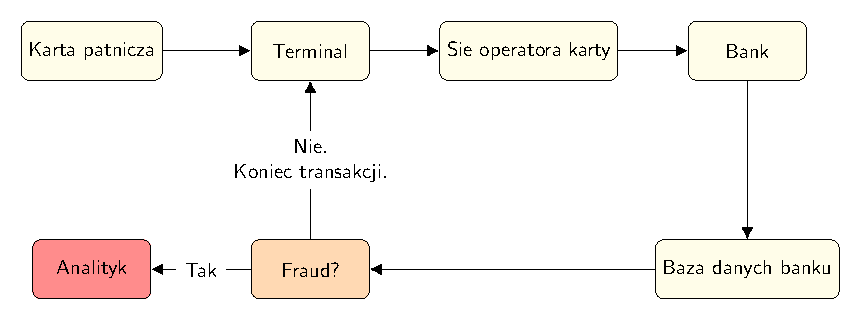
\includegraphics[width=\linewidth]{plots/transaction_schema.pdf}
	\caption{Schemat płatności kartą płatniczą. Źródło: Opracowanie własne na podstawie prezentacji A. Bahnsena~\cite{bahnsen_presentation}.}
	\label{fig:credit-card-flow}
\end{figure}

Banki oraz instytucje finansowe w celu przeciwdziałania tym przestępstwom korzystają z~systemów detekcji oszustw. Jest to jeden z elementów całego procesu dokonywania płatności, który jest przedstawiony na rysunku \ref{fig:credit-card-flow} na stronie \pageref{fig:credit-card-flow}. W~momencie przyłożenia karty kredytowej do terminala nawiązywane jest połączenie z operatorem karty (np. Visa, MasterCard), który dalej komunikuje się z bankiem klienta. Następnie w~odpowiednich bazach danych sprawdzane są dostępne środki, a~system detekcji oszustw sprawdza, czy transakcja nie jest podejrzana. W~przypadku wykrycia niezgodności system ją odrzuca i~kieruje sprawę do odpowiedniego analityka. W~przeciwnym razie płatność jest akceptowana i~na~terminalu wyświetla się odpowiedni komunikat.

Do niedawna najbardziej popularnym sposobem do wykrywania oszustw był system oparty na regułach eksperckich~\cite{bahnsen_presentation}. Powstawały one na bazie doświadczenia analityków, którzy podczas swojej długoletniej pracy wielokrotnie sprawdzali transakcje pod kątem oszustw i~byli w stanie dostrzec pewne zależności. Przykładami takich reguł mogą być: więcej niż cztery wypłaty z~bankomatu w~ciągu godziny, więcej niż dwie transakcje w~ciągu 5 minut, dwie transakcje w~ciągu 5 minut różnymi formami płatności (karta, internet). W przypadku, gdy rozpatrywana transakcja spełnia chociaż jedną z reguł, to jest ona blokowana i~użytkownik jest informowany o~odrzuceniu transakcji. To podejście jest stosunkowo łatwe do implementacji oraz bardzo proste do interpretacji, lecz niestety ma swoje wady. Przestępcy często wraz z~upływem czasu zmieniają swoje sposoby dokonywania oszustw, natomiast systemy złożone z~reguł eksperckich nie są w~stanie same wykrywać nowych zachowań i dostosowywać się do zmian, lecz wymagają do tego dodatkowej pracy analityków. Tę niedogodność są w~stanie rozwiązać modele uczenia maszynowego, które tworzą pewnego rodzaju reguły, które nie są bezpośrednio wprowadzane przez użytkownika, lecz automatycznie wykrywane przez algorytmy na podstawie dostarczonych danych historycznych. Wraz z~dynamicznym rozwojem tej dziedziny nauki zaczęły powstawać coraz bardziej wyrafinowane modele, które coraz lepiej radzą sobie z~wykrywaniem takich zależności. Obecnie są one już wykorzystywane w produkcyjnych środowiskach instytucji finansowych i~wspomagają walkę z~przestępcami \cite{practitioner_perspective}. Niestety standardowe podejście do modelowania predykcyjnego z wykorzystaniem uczenia maszynowego zakłada równy koszt popełnienia błędu, co nie jest założeniem odpowiadającym rzeczywistości. Stąd powstała motywacja do rozwoju metod, które biorą pod uwagę tę różnicę.

Celem pracy jest implementacja eksperymentu, który pozwoli porównać standardowe oraz wrażliwe na koszt metody predykcyjne w problemie detekcji oszustw na kartach płatniczych. Pierwszy rozdział zawiera wstęp teoretyczny, który wprowadzi odpowiednie pojęcia i~modele z dziedziny statystyki matematycznej oraz uczenia maszynowego. Następnie w~rozdziale drugim opiszemy przeprowadzone doświadczenie na danych rzeczywistych, w~którym zostały wykorzystane modele takie jak regresja logistyczna, drzewa decyzyjne, lasy losowe i~algorytm XGBoost wraz z~odpowiednimi modyfikacjami oraz metody optymalizacji progu i~minimalizacji ryzyka bayesowskiego. Ponadto rozdział zawiera omówienie otrzymanych rezultatów oraz wyciągniętych wniosków. Ostatnia część składa się z~podsumowania.

\chapter{Wprowadzenie teoretyczne}

Wprowadzenie teoretyczne zawiera przegląd metod z~dziedziny statystyki oraz uczenia maszynowego, które wykorzystuje się w~zagadnieniach klasyfikacyjnych. W~szczególności zostanie opisana macierz pomyłek, macierz kosztu oraz związane z nimi miary skuteczności modeli predykcyjnych, które służą do badania jakości predykcji. Następnie zostaną omówione modele standardowe, które nie biorą pod uwagi różnych kosztów popełniania błędu klasyfikacyjnego. W~ramach tej grupy zostanie opisana regresja logistyczna, drzewa decyzyjne, lasy losowe oraz algorytm XGBoost. Na końcu zostanie poruszony temat modeli wrażliwych na koszt, które dzielimy na dwie podkategorie: trening wrażliwy na koszt (\textit{ang. Cost Sensitive Training}) oraz klasyfikacja wrażliwa na koszt (\textit{ang. Cost Sensitive Classification}) \cite{RMoser}. Pierwsza z nich zawiera metody, które w trakcie uczenia modelu zwracają uwagę na koszt błędnej klasyfikacji. Są to rozszerzone wersje standardowych modeli, które w~trakcie uczenia się mają zmienioną postać optymalizowanej funkcji. W~niniejszej pracy będziemy omawiać regresję logistyczną wrażliwą na koszt oraz drzewa decyzyjne wrażliwe na koszt. Druga podkategoria składa się z~metod, które wykorzystują estymowane prawdopodobieństwo ze~standardowych modeli i~na jego podstawie tworzą dodatkowy model, który bierze pod uwagę koszt niepoprawnej klasyfikacji danego przypadku. Z~tej grupy zostanie omówiona optymalizacja progu oraz minimalizacja ryzyka bayesowskiego.

W pracy wykorzysytwane są następujące oznaczenia:
\begin{itemize}
	\item $\es = \{\iks_1, \iks_2, \dots, \iks_N \}$ -- zbiór wszystkich $N$ obserwacji,
	\item $\iks_{i} = \left(x_i^{(1)}, x_i^{(2)}, \dots, x_i^{(j)} \right)$ -- $i$-ty wektor obserwacji składający się z $j$ atrybutów,
	\item $x_i^{(k)}$ -- $k$-ty atrybut $i$-tego wektora obserwacji,
	\item $\ytrue = (y_1, y_2, \dots, y_N)$ -- wektor prawdziwych stanów klasyfikacji,
	\item $y_i \in \{0,1\}$ -- prawdziwy stan klasyfikacji dla $i$-tej obserwacji,
	\item $\boldsymbol{p} = (p_1, p_2, \dots, p_N)$ -- wektor estymowanych wartość prawdopodobieństwa,
	\item $p_i = P(y_i = 1 | \es)$ -- estymowana wartość prawdopodobieństwa dla $i$-tej obserwacji,
	\item $\boldsymbol{c} = (c_1, c_2, \dots, c_N) $ -- wektor przewidywanych klas,
	\item $c_i \in \{0,1\} $ -- przewidywana klasa dla $i$-tej obserwacji.
\end{itemize}
Wartość $y_i = 0$ oznacza wartość niesprzyjającą a $y_i = 1$ sprzyjającą. Ponadto $c_i = 0$ oznacza klasyfikację negatywną, natomiast $c_i = 1$ pozytywną.

\section{Miary skuteczności modeli}

\subsection{Macierz pomyłek}

Jedną z metod wykorzystywanych do oceny skuteczności modeli w zadaniach klasyfikacyjnych jest macierz pomyłek. Prawidłowe stany zestawiamy z klasami nadanymi przez model, a~następnie sprawdzamy, czy poprawnie zaklasyfikowaliśmy poszczególne obserwacje. W~przypadku klasyfikacji binarnej popełniamy dwa rodzaje błędów, a~wszystkie możliwe wyniki prezentują się w~następujący sposób:
\begin{itemize}
	\item[--] Prawdziwie pozytywny wynik klasyfikacji (TP, z angielskiego \textit{True Positive}) -- obserwacja miała stan sprzyjający i zaklasyfikowaliśmy ją jako pozytywną;
	\item[--] Fałszywie pozytywny wynik klasyfikacji (FP, z angielskiego \textit{False Positive}) -- obserwacja miała stan niesprzyjający i zaklasyfikowaliśmy ją jako pozytywną. W~nomenklaturze statystycznej nazywamy ją również błędem pierwszego rodzaju;
	\item[--] Fałszywie negatywny wynik klasyfikacji (FN, z angielskiego \textit{False Negative}) -- obserwacja miała stan sprzyjający i zaklasyfikowaliśmy ją jako negatywną. W~nomenklaturze statystycznej nazywamy ją również błędem drugiego rodzaju;
	\item[--] Prawdziwie negatywny wynik klasyfikacji (TN, z angielskiego \textit{True Negative}) -- obserwacja miała stan niesprzyjający i zaklasyfikowaliśmy ją jako negatywną.
\end{itemize}
\noindent Liczbę obserwacji należących do poszczególnych kategorii możemy reprezentować tak jak w~tabeli \ref{tab:macierz-pomylek}, gdzie
\begin{itemize}
	\item TP $ = \#\{i: i \in \{1,\dots,N\}, y_i = c_i = 1\}$,
	\item FP $ = \#\{i: i \in \{1,\dots,N\}, y_i = 0, c_i = 1\}$,
	\item FN $ = \#\{i: i \in \{1,\dots,N\}, y_i = 1, c_i = 0\}$,
	\item TN $ = \#\{i: i \in \{1,\dots,N\}, y_i = c_i = 0\}$.
\end{itemize}

\begin{table}[h]
	\begin{center}
%		\renewcommand{\arraystretch}{1.2}
		\begin{tabular}{c|c|c}
			 \multirow{2}{8em}{} & Stan sprzyjający & Stan niesprzyjający \\
			                  & $y_i = 1$            & $y_i = 0$ \\
			 \hline
			  Predykcja pozytywna & \multirow{2}{8em}{\centering TP}& \multirow{2}{8em}{\centering FP} \\
			    $c_i = 1$ &  &                 \\
			 \hline
			 Predykcja negatywna & \multirow{2}{8em}{\centering FN} & \multirow{2}{8em}{\centering TN} \\
			   $c_i = 0$ &  &  \\
		\end{tabular}
	\end{center}
	\caption{Macierz pomyłek.}
	\label{tab:macierz-pomylek}
\end{table}

\subsection{Miary skuteczności niewrażliwe na koszt}
Na podstawie macierzy pomyłek (tabela \ref{tab:macierz-pomylek}) możemy zdefiniować następujące miary skuteczności modeli, które nie biorą pod uwagę kosztu popełnienia błędu. Przytoczone definicje pochodzą z~pracy D. Powersa \cite{evaluation_metrics}.

\subsubsection{Precyzja}
Precyzja (\textit{ang. Precision}) to stosunek poprawnie zaklasyfikowanych pozytywnych przypadków do wszystkich obserwacji zaklasyfikowanych jako pozytywne. Mierzy ona, jaki procent próbek prawidłowo zaklasyfikowaliśmy jako pozytywne. Warto zauważyć, że nie bierze ona pod uwagę klasyfikacji negatywnych. Jest ona bardzo często wykorzystywana podczas rozwiązywania większości problemów z~zakresu uczenia maszynowego, ponieważ najczęściej interesuje nas, aby nasze typowania były możliwie najbardziej skuteczne. Z~tego też powodu precyzja jest często nazywana skutecznością klasyfikacji prawdziwie pozytywnych (\textit{ang. True Positive Accuracy}). Zapisana wzorem przyjmuje postać
$$ \text{Precyzja} = \frac{TP}{TP + FP} \text{.}$$
Rozpatrzmy jeszcze przykład z~medycyny. Załóżmy, że mamy test diagnostyczny, który klasyfikuje wszystkich pacjentów jako chorych. W~tym przypadku czułość przyjmuje wartość $1$, swoistość wartość $0$, a precyzja jest równa frakcji przypadków pozytywnych w danych. Odwrotnie, załóżmy teraz, że nasz test oznacza wszystkich pacjentów jako zdrowych. W~tym przypadku czułość jest równa $0$, swoistość $1$, natomiast precyzja jest niezdefiniowana (symbol nieoznaczony -- $\frac{0}{0}$). Ten przykład pokazuje, że precyzja jest zależna od zbalansowania klas.

\subsubsection{Czułość}
Czułość (\textit{ang. Recall} lub \textit{ang. Sensitivity}) to stosunek prawdziwie pozytywnie zaklasyfikowanych przypadków do wszystkich sprzyjających obserwacji. Innymi słowy, jest to miara, która mówi nam o procencie znalezionych przez model przypadków sprzyjających. Podobnie jak precyzja skupia się jedynie na poprawnie zaklasyfikowanych obserwacjach pozytywnych. Jest ona szczególnie ważna w zastosowaniach medycznych, gdzie naszym głównym celem jest znalezienie wszystkich chorych osób. Używana jest także do wyznaczania krzywej ROC. Czułość jest wyrażona wzorem
$$ \text{Czułość}= \frac{TP}{TP + FN} \text{.}$$

\subsubsection{Swoistość}
Swoistość (\textit{ang. Specificity}) to stosunek prawdziwie negatywnie zaklasyfikowanych przypadków do wszystkich niesprzyjających obserwacji. Inaczej nazywana też odwrotną czułością, gdyż podobnie do czułości mierzy ona odsetek znalezionych wszystkich obserwacji, lecz dla negatywnej klasy. Miara ta jest także używana do wyrysowania krzywej ROC, a dokładniej wartość $1- \text{Swoistość}$, która odpowiada stosunkowi fałszywie pozytywnych klasyfikacji (ang. \textit{false positive ratio}). Swoistość wyraża się następującym wzorem
$$ \text{Swoistość}= \frac{TN}{TN + FP} \text{.}$$

\subsubsection{Dokładność}
Dokładność (\textit{ang. Accuracy}) mierzy stosunek poprawnie zaklasyfikowanych przypadków do ilości wszystkich obserwacji. Bierze ona pod uwagę zarówno obserwacje pozytywne, jak i negatywne. Z~tego powodu bardzo dobrze radzi sobie w sytuacji, gdy interesują nas obserwacje z obu klas, natomiast dużo gorzej, gdy istotna jest tylko jedna klasa. W~szczególności nie nadaje się ona do problemów z dużą dysproporcją klas, która pojawia się w przypadku detekcji oszustw. Dokładność zdefiniowana jest następującym wzorem
$$ \text{Dokładność} = \frac{TP + TN}{TP + FP + FN + TN} \text{,}$$
który możemy zapisać również jako (wyprowadzenie w dodatku \ref{dokladnosc-dd})
\begin{equation}
	\label{dokl}
	\text{Dokładność} = \alpha \cdot \text{Czułość} + (1-\alpha) \cdot \text{Swoistość} \text{,}
\end{equation}
gdzie $\alpha$ to odsetek przypadków sprzyjających w~danych.

Rozpatrzmy pewien przykład. Załóżmy, że mamy dwóch naukowców, którzy posługują się tą samą metodą w badaniach, lecz mają oni różne proporcje stanów w populacji. W~tym przypadku otrzymają oni różną dokładność, mimo tego, że wyniki nie powinny się różnić z~uwagi na korzystanie z~tej samej metody. W~celu uniknięcia takiej sytuacji możemy wykorzystać miarę zbalansowanej skuteczność (\textit{BACC, ang. balanced accuracy}). Dana jest ona wzorem \ref{dokl}, gdzie za parametr $\alpha$ przyjmuje się wartość $\frac{1}{2}$. W~przypadku, gdy mamy równe proporcje klas, to sprowadza się ona do dokładności, natomiast gdy standardowa dokładność jest wysoka tylko z uwagi na niezbalansowaną liczność próbek w klasach, to wartość zbalansowanej skuteczności spada \cite{balanced_accuracy}. Jest ona również ważna, ponieważ maksymalizacja tej miary odpowiada standardowemu szukaniu optymalnego punktu na krzywej ROC według metryki taksówkowej.

\subsubsection{Krzywa ROC}

Krzywa ROC to wykres diagnostyczny modelu predykcyjnego pozwalający na zilustrowanie jakości predykcyjnej klasyfikatora. Składa się ona z wyrysowanym na osi X stosunku fałszywie pozytywnych klasyfikacji oraz czułości na osi Y \cite{evaluation_metrics}. Miary są narysowane dla różnych wartości progu decyzyjnego, który prawdopodobieństwa zwracane przez model zamienia na decyzje binarne. Perfekcyjny klasyfikator jest w~stanie osiągnąć lewy górny róg wykresu, czyli posiadać precyzję na poziomie 100\% oraz stosunek fałszywie pozytywnych klasyfikacji na poziomie 0\%. Inaczej, taki model ma czułość oraz precyzję na poziomie 100\%, a co za tym idzie 100\% dokładność, a to oznacza, że nigdy się nie myli.  Analogicznie najgorszy klasyfikator jest w stanie osiągnąć prawy dolny róg wykresu. Modelem losowy będzie punkt na prostej z punktu $(0,0)$ do punktu $(1,1)$, czyli każda dowolna klasyfikacja z rozkładu $B(1, p)$ niezależnego od $X$ jest w punkcie $(p, p)$. Ponadto warto zauważyć, że klasyfikatory z~przykładu w~sekcji dotyczącej precyzji (wszyscy chorzy i~wszyscy zdrowi) też tutaj są -- na końcach tego odcinka w~punkcie $(1, 1)$ oraz $(0, 0)$ odpowiednio.

Przykładowy wykres znajduje się na rysunku \ref{fig:roc_example} na stronie \pageref{fig:roc_example}. Kolorem czerwonym oznaczony jest najgorszy możliwy klasyfikator, zielonym perfekcyjny, niebieskim losowy, natomiast żółtym przykładowy.

\begin{figure}[h]
	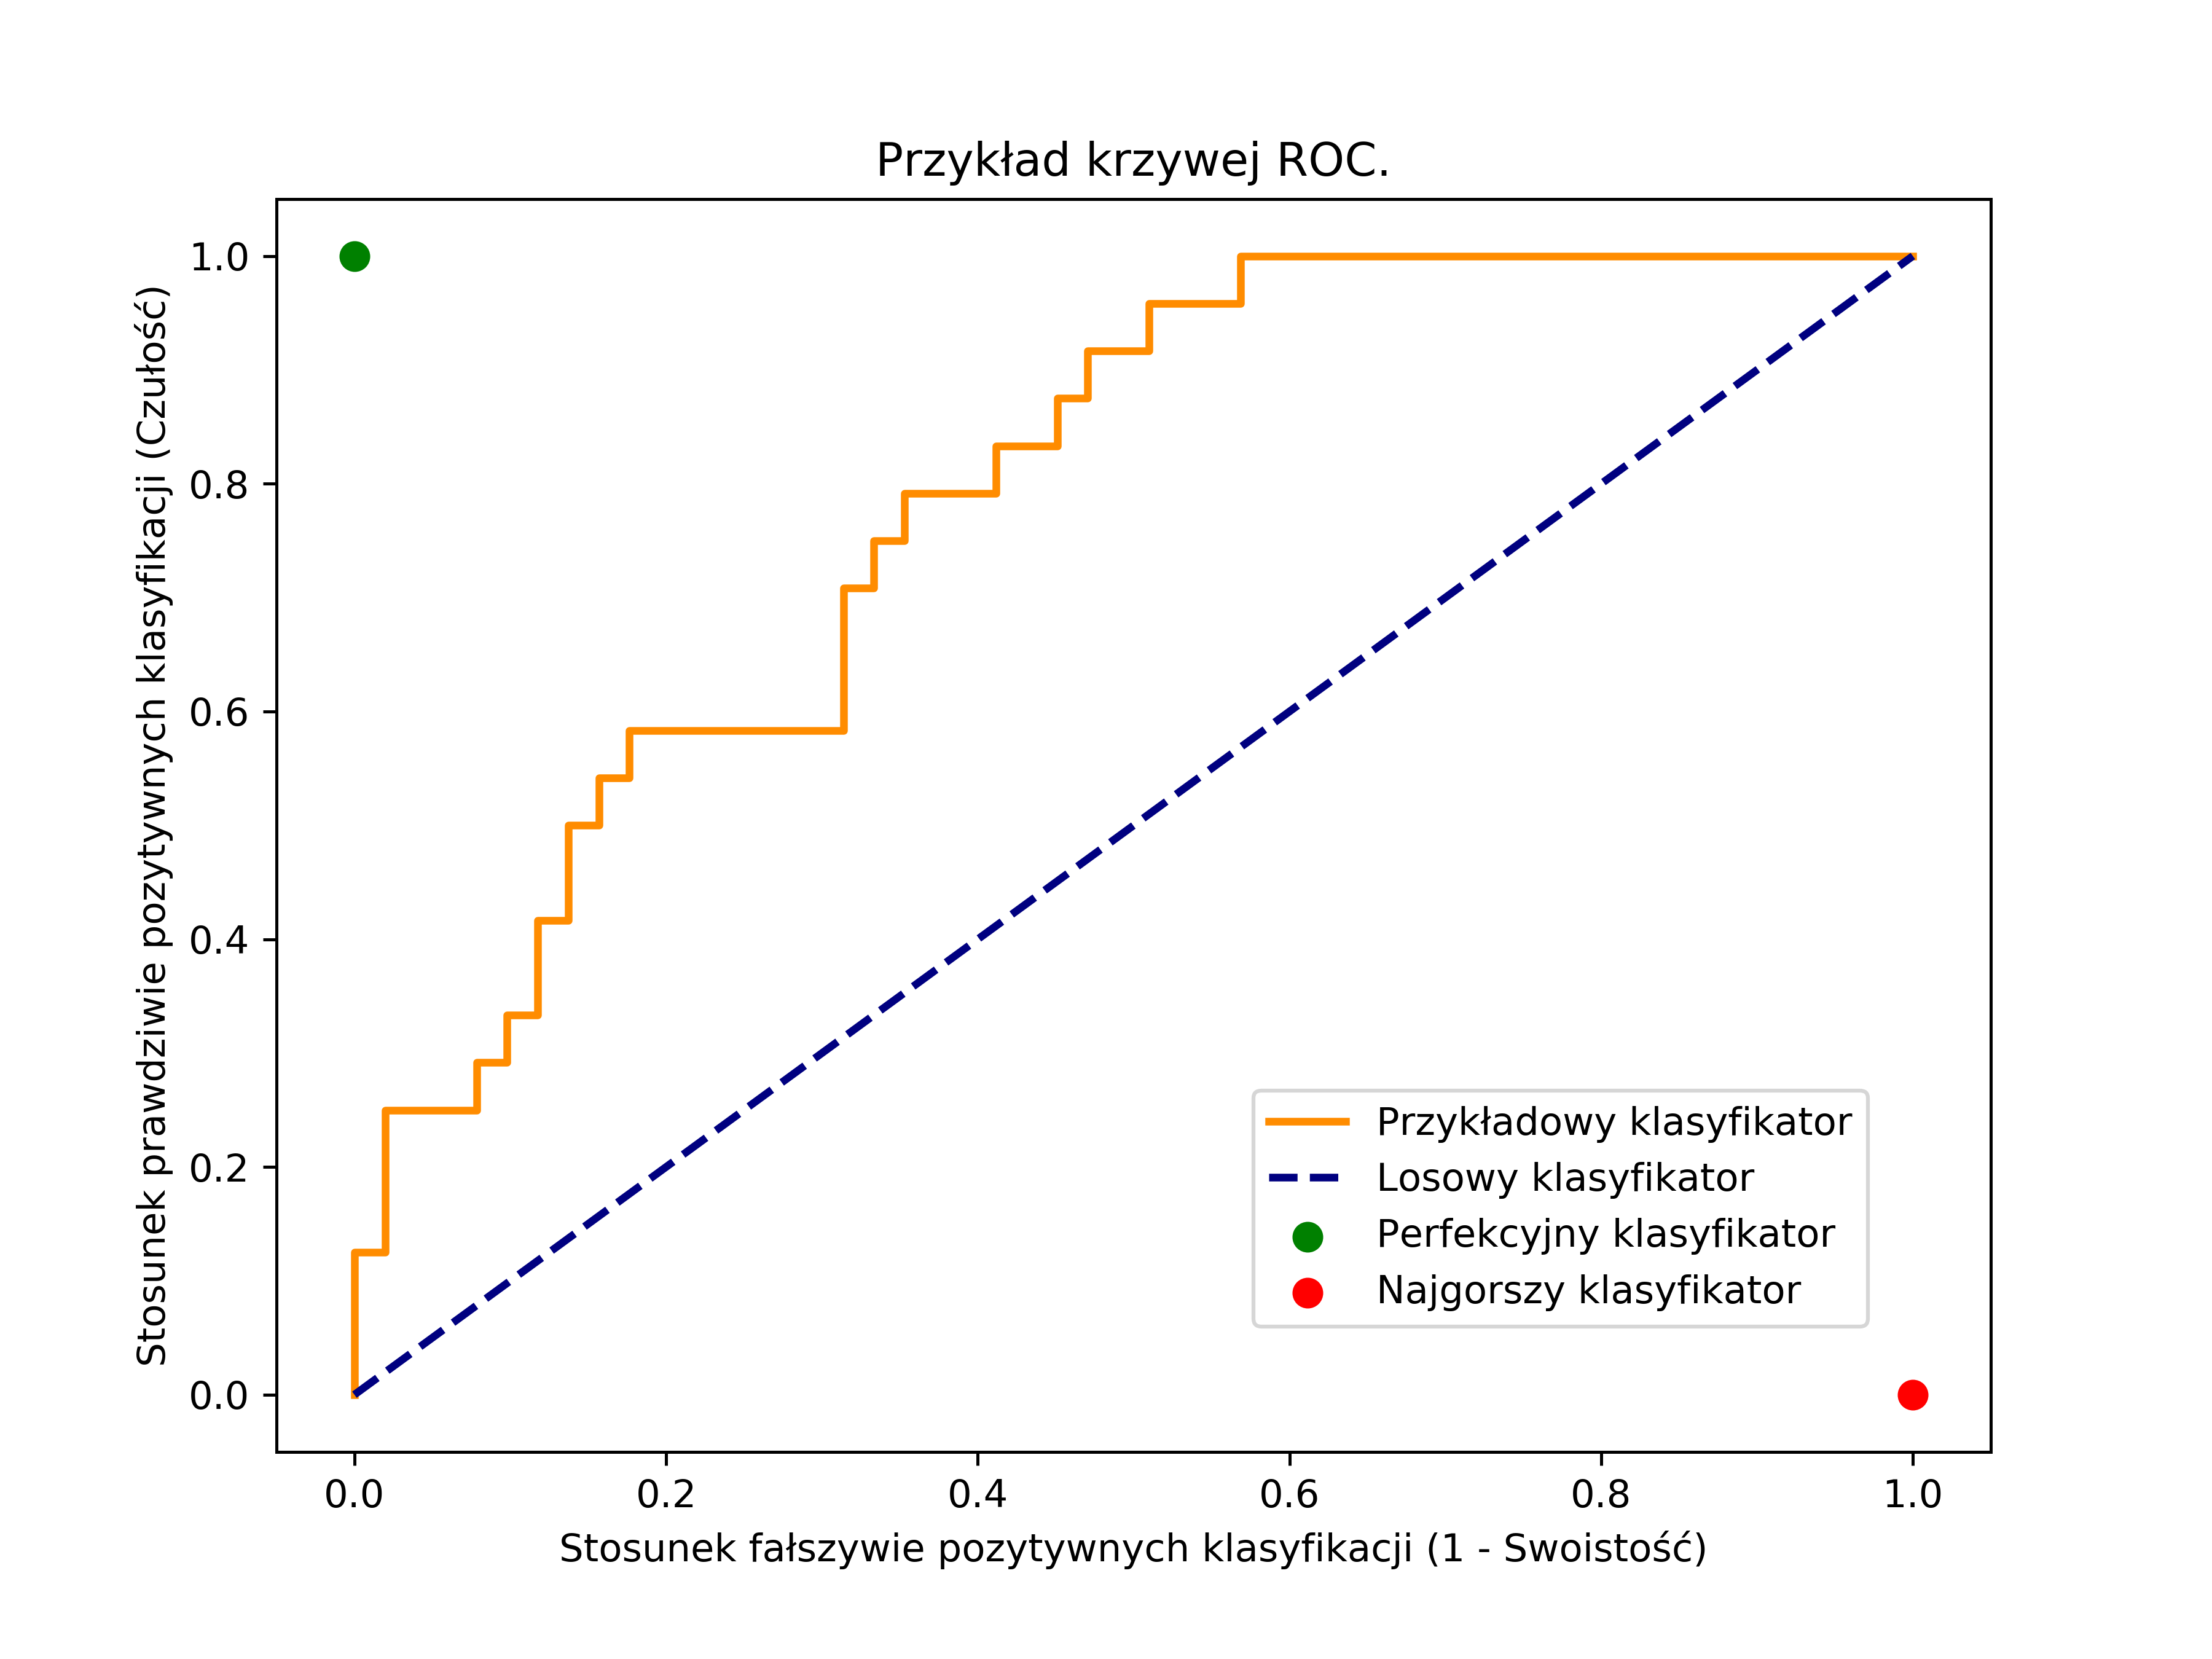
\includegraphics[width=\linewidth]{images/roc_example.png}
	\caption{Przykładowy wykres charakterystyki pracy odbiornika. Na poziomej osi przedstawiony jest stosunek fałszywie pozytywnych klasyfikacji, natomiast na pionowej czułość. Kolorem czerwonym, zielonym, niebieskim oraz żółtym jest odpowiednio oznaczony najgorszy, najlepszy, losowy oraz przykładowy klasyfikator. Źródło: Opracowanie własne.}
	\label{fig:roc_example}
\end{figure}

Celem tworzenia oraz ulepszania kolejnych modeli predykcyjnych jest zbliżanie się w~wynikach do lewego górnego rogu wykresu. Odległość danego punktu reprezentującego konkretny model możemy definiować w różnych metrykach. Przykładowo w metryce taksówkowej (metryka $L_1$) będzie to 
$$ 1 - \text{Swoistość} + 1 - \text{Czułość} \text{.}$$
Dokonując kolejne przekształcenia otrzymujemy
\begin{equation*}
\begin{split}
 1 - \text{Swoistość} + 1 - \text{Czułość} & = 2 - (\text{Czułość} + \text{Swoistość}) = \\
& = 2 \cdot (1 - (\text{Czułość} + \text{Swoistość})/2) = 2 \cdot (1 - \text{BACC}) \text{.}
\end{split}
\end{equation*}
Oznacza to, że im większa zbalansowana skuteczność danego modelu, tym bliżej znajduje się model na krzywej ROC lewego górnego rogu. W podobny sposób możemy także rozważać inne metryki. Przykładowo w metryce euklidesowej (metryka $L_2$) będziemy chcieli minimalizować następujące wyrażenie
$$ \sqrt{(1 - \text{Swoistość})^2 + (1 - \text{Czułość})^2} \text{,}$$
bądź ogólniej w metryce $L_p$
$$ \big( (1 - \text{Swoistość})^p + (1 - \text{Czułość})^p \big)^{\frac{1}{p}} \text{.} $$

\subsubsection{F Score}
$\text{F}_1$ Score to miara łącząca w sobie precyzję oraz czułość za pomocą średniej harmonicznej. Z~uwagi na wykorzystanie tych dwóch wartości nie bierze ona pod uwagę prawidłowo zaklasyfikowanych obserwacji negatywnych. Wykorzystanie średniej harmonicznej powoduje, że kładziemy równy nacisk na obie użyte miary. Standardowy wzór wygląda następująco
$$ F_1 = \left(\frac{2}{\text{Precyzja}^{-1} + \text{Czułość}^{-1}}\right) = 2 \cdot \frac{\text{Precyzja} \cdot \text{Czułość}}{\text{Precyzja} + \text{Czułość}} \text{.}$$

W przypadku, gdy interesuje nas bardziej precyzja lub czułość, to definiujemy bardziej ogólną formułę na $\text{F}_{\beta}$ Score:
$$ F_{\beta} = (1 + \beta^2) \cdot \frac{\text{Precyzja} \cdot \text{Czułość}}{(\beta^2 \cdot \text{Czułość}) + \text{Precyzja}} \text{,}$$
gdzie parametr $\beta>0$ odpowiada na pytanie, ile razy bardziej czułość jest ważna niż precyzja. Najczęściej wykorzystuje się parametr $\beta = 2$ lub $\beta = \frac{1}{2}$, który odpowiednio zwiększa nacisk na czułość lub zmniejsza wpływ fałszywie negatywnie zaklasyfikowanych obserwacji, skupiając się bardziej na precyzji.

\subsection{Macierz kosztu}
\label{sec:macierz-kosztu}
W celu wprowadzenia potrzebnych miar skuteczności wrażliwych na koszt, musimy zdefiniować wektor macierzy kosztu
$$ \boldsymbol{C} = (C_1, C_2, \dots, C_N) $$
gdzie $ C^{(i)} = [C^{(i)}_{j,k}]_{j,k=0}^1 $ oznacza macierz kosztu dla $i$-tej obserwacji \cite{CSCCFD, CS-Learning}. Ma ona postać analogiczną do macierzy pomyłek, lecz zamiast ilości obserwacji w odpowiednich komórkach wpisujemy koszt pomyłki dla $i$-tej obserwacji. Warto zaznaczyć, że koszt niekoniecznie musi być kwota pieniężną, lecz także możemy rozważać ilość poświęconego czasu, bądź inną dowolną mierzalną jednostkę. W szczególności dla przypadku klasyfikacji binarnej wyróżniamy cztery możliwe wartości:
\begin{itemize}
	\item[--] $C^{(i)}_{1,1}$ -- koszt prawdziwie pozytywnego zaklasyfikowania $i$-tej obserwacji,
	\item[--] $C^{(i)}_{1,0}$ -- koszt fałszywie pozytywnego zaklasyfikowania $i$-tej obserwacji,
	\item[--] $C^{(i)}_{0,1}$ -- koszt fałszywie negatywnego zaklasyfikowania $i$-tej obserwacji,
	\item[--] $C^{(i)}_{0,0}$ -- koszt prawdziwie negatywnego zaklasyfikowania $i$-tej obserwacji.
\end{itemize}

W zależności od praktycznego zastosowania wartości w macierzy kosztu przyjmują różne wielkości. Poniżej przedstawiamy kilka intuicji na podstawie macierzy kosztu zdefiniowanych dla różnych eksperymentów w~pracy A. Bahnsena \cite{alej2015ensemble}.
\begin{itemize}
	\item W przypadku, gdy predykcja klasy pozytywnej wiąże się z podjęciem jakiejś akcji, np. sprawdzenie transakcji kartą kredytową, wysłanie oferty reklamowej, to koszt pozytywnej predykcji jest dodatni, to znaczy $C^{(i)}_{1,1}$, $C^{(i)}_{1,0}$ $>0$. Ponadto najczęściej te koszty są równe i przyjmują stałą wartość dla wszystkich przypadków, to znaczy $C^{(i)}_{1,1} = C^{(i)}_{1,0} =  \text{const.}$, ponieważ podejmowana zawsze jest ta sama akcja dla wszystkich obserwacji. Dodatkowo koszt pozytywnego zaklasyfikowania dla każdej obserwacji negatywnej jest zerowy, to znaczy $C^{(i)}_{0,0} = 0$, ponieważ słusznie nie została podjęta żadna akcja. Zatem ostatecznie jedyną wartością, która różni się między przypadkami, jest koszt fałszywie negatywnej klasyfikacji i on również jest większy od zera.
	\item W~przypadku, gdy predykcja dokonywana jest przez zautomatyzowany system, to koszt prawidłowej klasyfikacji jest równy zero, to znaczy $C^{(i)}_{1,1} = C^{(i)}_{0,0} = 0$. Jest to spowodowane faktem, że maszynie nie musimy płacić pensji, a~koszt czasowy i~sprzętowy jest pomijalny. Natomiast koszty pomyłek są inne i~zazwyczaj różnią się między obserwacjami. Biorąc jako przykład ryzyko kredytowe, możemy zauważyć, że koszty mogą być zarówno dodatnie, jak i ujemne. W tym konkretnym przypadku, gdy stwierdzimy, że dana osoba spłaci kredyt, natomiast w rzeczywistości nie zrobi tego, to będziemy stratni pewną sumę pieniędzy, co da nam dodatni koszt. Z~drugiej strony, gdy uznamy, że dana osoba nie spłaci kredytu, a w rzeczywistości wywiązałaby się ze zobowiązań, to utracimy pewien zarobek, zatem koszt będzie ujemny.
\end{itemize}

Koncepcyjnie koszt popełnienia błędu dla każdej obserwacji powinien być większy niż koszt poprawnej klasyfikacji, to znaczy

$$ C^{(i)}_{1,0} > C^{(i)}_{1,1} \text{ i } C^{(i)}_{0,1} > C^{(i)}_{0,0} \quad \forall_{i \in \{1, 2, \dots, N\}} \text{.}$$

Ilustracja takiej macierzy kosztu znajduje się w tabeli \ref{tab:macierz-kosztu}.
\begin{table}[h]
	\begin{center}
		\begin{tabular}{c|c|c}
			\multirow{2}{4em}{} & Stan pozytywny & Stan negatywny \\
			& $y_i = 1$            & $y_i = 0$ \\
			\hline
			Predykcja pozytywna & \multirow{2}{4em}{\centering $C^{(i)}_{1,1}$} & \multirow{2}{4em}{\centering $C^{(i)}_{1,0}$} \\
			$c_i = 1$         &                    &                    \\
			\hline
			Predykcja negatywna & \multirow{2}{4em}{\centering $C^{(i)}_{0,1}$} & \multirow{2}{4em}{\centering $C^{(i)}_{0,0}$} \\
			$c_i = 0$         &                    &                    \\
		\end{tabular}
	\end{center}
	\caption{Macierz kosztu dla $i$-tej obserwacji.}
	\label{tab:macierz-kosztu}
\end{table}

\subsection{Miary skuteczności modeli wrażliwych na koszt}
Motywacją do powstania miar skuteczności wrażliwych na koszt jest potrzeba ewaluacji modeli, która miarodajnie odda złożoność rozwiązywanego problemu \cite{EDCSLR}. Przykładowo w~przypadku detekcji oszustw będzie w stanie odpowiedzieć na pytanie dotyczące zaoszczędzonej kwoty dzięki modelowi predykcyjnemu. Kolejny powodem jest fakt, że podstawowe metryki nie uwzględniają różnicy w kosztach pomyłki dla fałszywie pozytywnych oraz fałszywie negatywnych klasyfikacji, traktując oba błędy jednakowo. Ponadto warto zauważyć, że omawiane problemy wymagają uwzględnienia nie tylko różnych kosztów dla każdego rodzaj pomyłki, ale także każdej konkretnej obserwacji. Bazując na wprowadzonym w~sekcji \ref{sec:macierz-kosztu} wektorze macierzy kosztu $C$, można zdefiniować następujące miary.

\subsubsection{Koszt całkowity}
Koszt całkowity (TC, z angielskiego \textit{ang. Total Cost}) to suma kosztów poniesionych dla danego zestawu predykcji $\boldsymbol{c}$, który zostały wygenerowany przez pewien model predykcyjny. Definiowany jest wzorem
\begin{equation}
	\label{koszt-calkowity}
	\text{TC}(\ytrue, \boldsymbol{c}, \boldsymbol{C}) = \sum_{i=1}^N C^{(i)}_{c_i,y_i} \text{.}
\end{equation} 

\subsubsection{Oszczędności}
Oszczędności (\textit{ang. Savings}) to miara, którą intuicyjnie możemy rozumieć jako procentową wartość, o~ile testowany model jest lepszy od naiwnego klasyfikatora. Przy czym naiwnym klasyfikatorem nazywamy model, który zwraca same predykcje pozytywne lub same predykcje negatywne, w~zależności od tego, co bardziej się opłaca dla danego zestawu danych.
\begin{equation}
	\label{oszczednosci}
	\text{Oszczędności}(\ytrue, \boldsymbol{c}, \boldsymbol{C}) = \frac{\text{Koszt bazowy}(\ytrue, \boldsymbol{C}) - \text{TC}(\ytrue, \boldsymbol{c}, \boldsymbol{C})}{\text{Koszt bazowy}(\ytrue, \boldsymbol{C})} \text{,}
\end{equation}
gdzie:
\begin{itemize}
	\item $ \text{koszt bazowy}(\ytrue, \boldsymbol{C}) = \min\{\text{TC}(\ytrue, \boldsymbol{c}_0, \boldsymbol{C}), \text{TC}(\ytrue, \boldsymbol{c}_1, \boldsymbol{C})\} \neq 0$ -- koszt poniesiony w~przypadku używania naiwnego klasyfikatora,
	\item $\boldsymbol{c}_0 = (0, 0, \dots, 0)$ -- $N$-elementowy wektor predykcji równych $0$,
	\item $\boldsymbol{c}_1 = (1, 1, \dots, 1)$ -- $N$-elementowy wektor predykcji równych $1$.
\end{itemize}{}

\section{Standardowe modele}

\subsection{Regresja logistyczna}
\label{reg-log}
Regresja logistyczna to model statystyczny, którego celem jest modelowanie prawdopodobieństwa, że zmienna losowa $Y$ przyjmie wartość $0$ lub $1$, na~podstawie danych empirycznych. Rozważmy następującą definicję modelu regresji logistycznej parametryzowaną wektorem współczynników $\theta = (\theta_1, \theta_2, \dots, \theta_n)$ daną w~następujący sposób
\begin{equation}
	\htx = \frac{1}{1+e^{-\iks_{i}\theta^T}} = P(Y = 1|X = \iks_{i};\theta) \text{.}
\end{equation} 
Jednocześnie zauważmy, że
$$ P(Y = 0|X = \iks_{i};\theta) = 1 - P(Y = 1|X = \iks_{i};\theta) = 1 - \htx $$
oraz korzystając z faktu, że $y_i \in \{0,1\}$, możemy zapisać 
$$ P(Y = y_i|X = \iks_{i};\theta) = \htx^{y_i}(1-\htx)^{(1-y_i)} \text{.}$$
Następnie wyznaczamy funkcję wiarogodności, aby wyestymować parametry~$\theta$.
$$ L(\theta | \es, \ytrue) = \prod_{i=1}^N P(Y = y_i | X = \iks_{i}; \theta) = \prod_{i=1}^N \htx^{y_i}(1-\htx)^{(1-y_i)} \text{.}$$
W celu znalezienia maksimum funkcji wiarogodności logarytmujemy funkcję $L(\theta | \es, \ytrue)$ i~otrzymujemy funkcję logarytmu wiarogodności $l(\theta | \es, \ytrue)$
$$ l(\theta | \es, \ytrue) = \log L(\theta | \es, \ytrue)  = -\sum_{i=1}^N J_i(\theta) \text{,}$$
gdzie $J_i(\theta)$ nazywana jest entropią krzyżową i przyjmuje postać
\begin{equation}
	\label{c-e}
	J_i(\theta) = -\big(y_i\log(h_{\theta}(\boldsymbol{x_i})) + (1-y_i)\log(1 - h_{\theta}(\boldsymbol{x_i}))\big) \text{.}
\end{equation}
Niestety nie jest możliwe znalezienie bezpośredniego wzoru na współczynniki, które maksymalizują funkcję logarytmu wiarogodności $l(\theta | \es, \ytrue)$, zatem wykorzystuje się w~tym celu algorytmy optymalizacji numerycznej, np. IRLS (\textit{ang. Iteratively Reweighted Least Squares}).

\begin{figure}[h]
	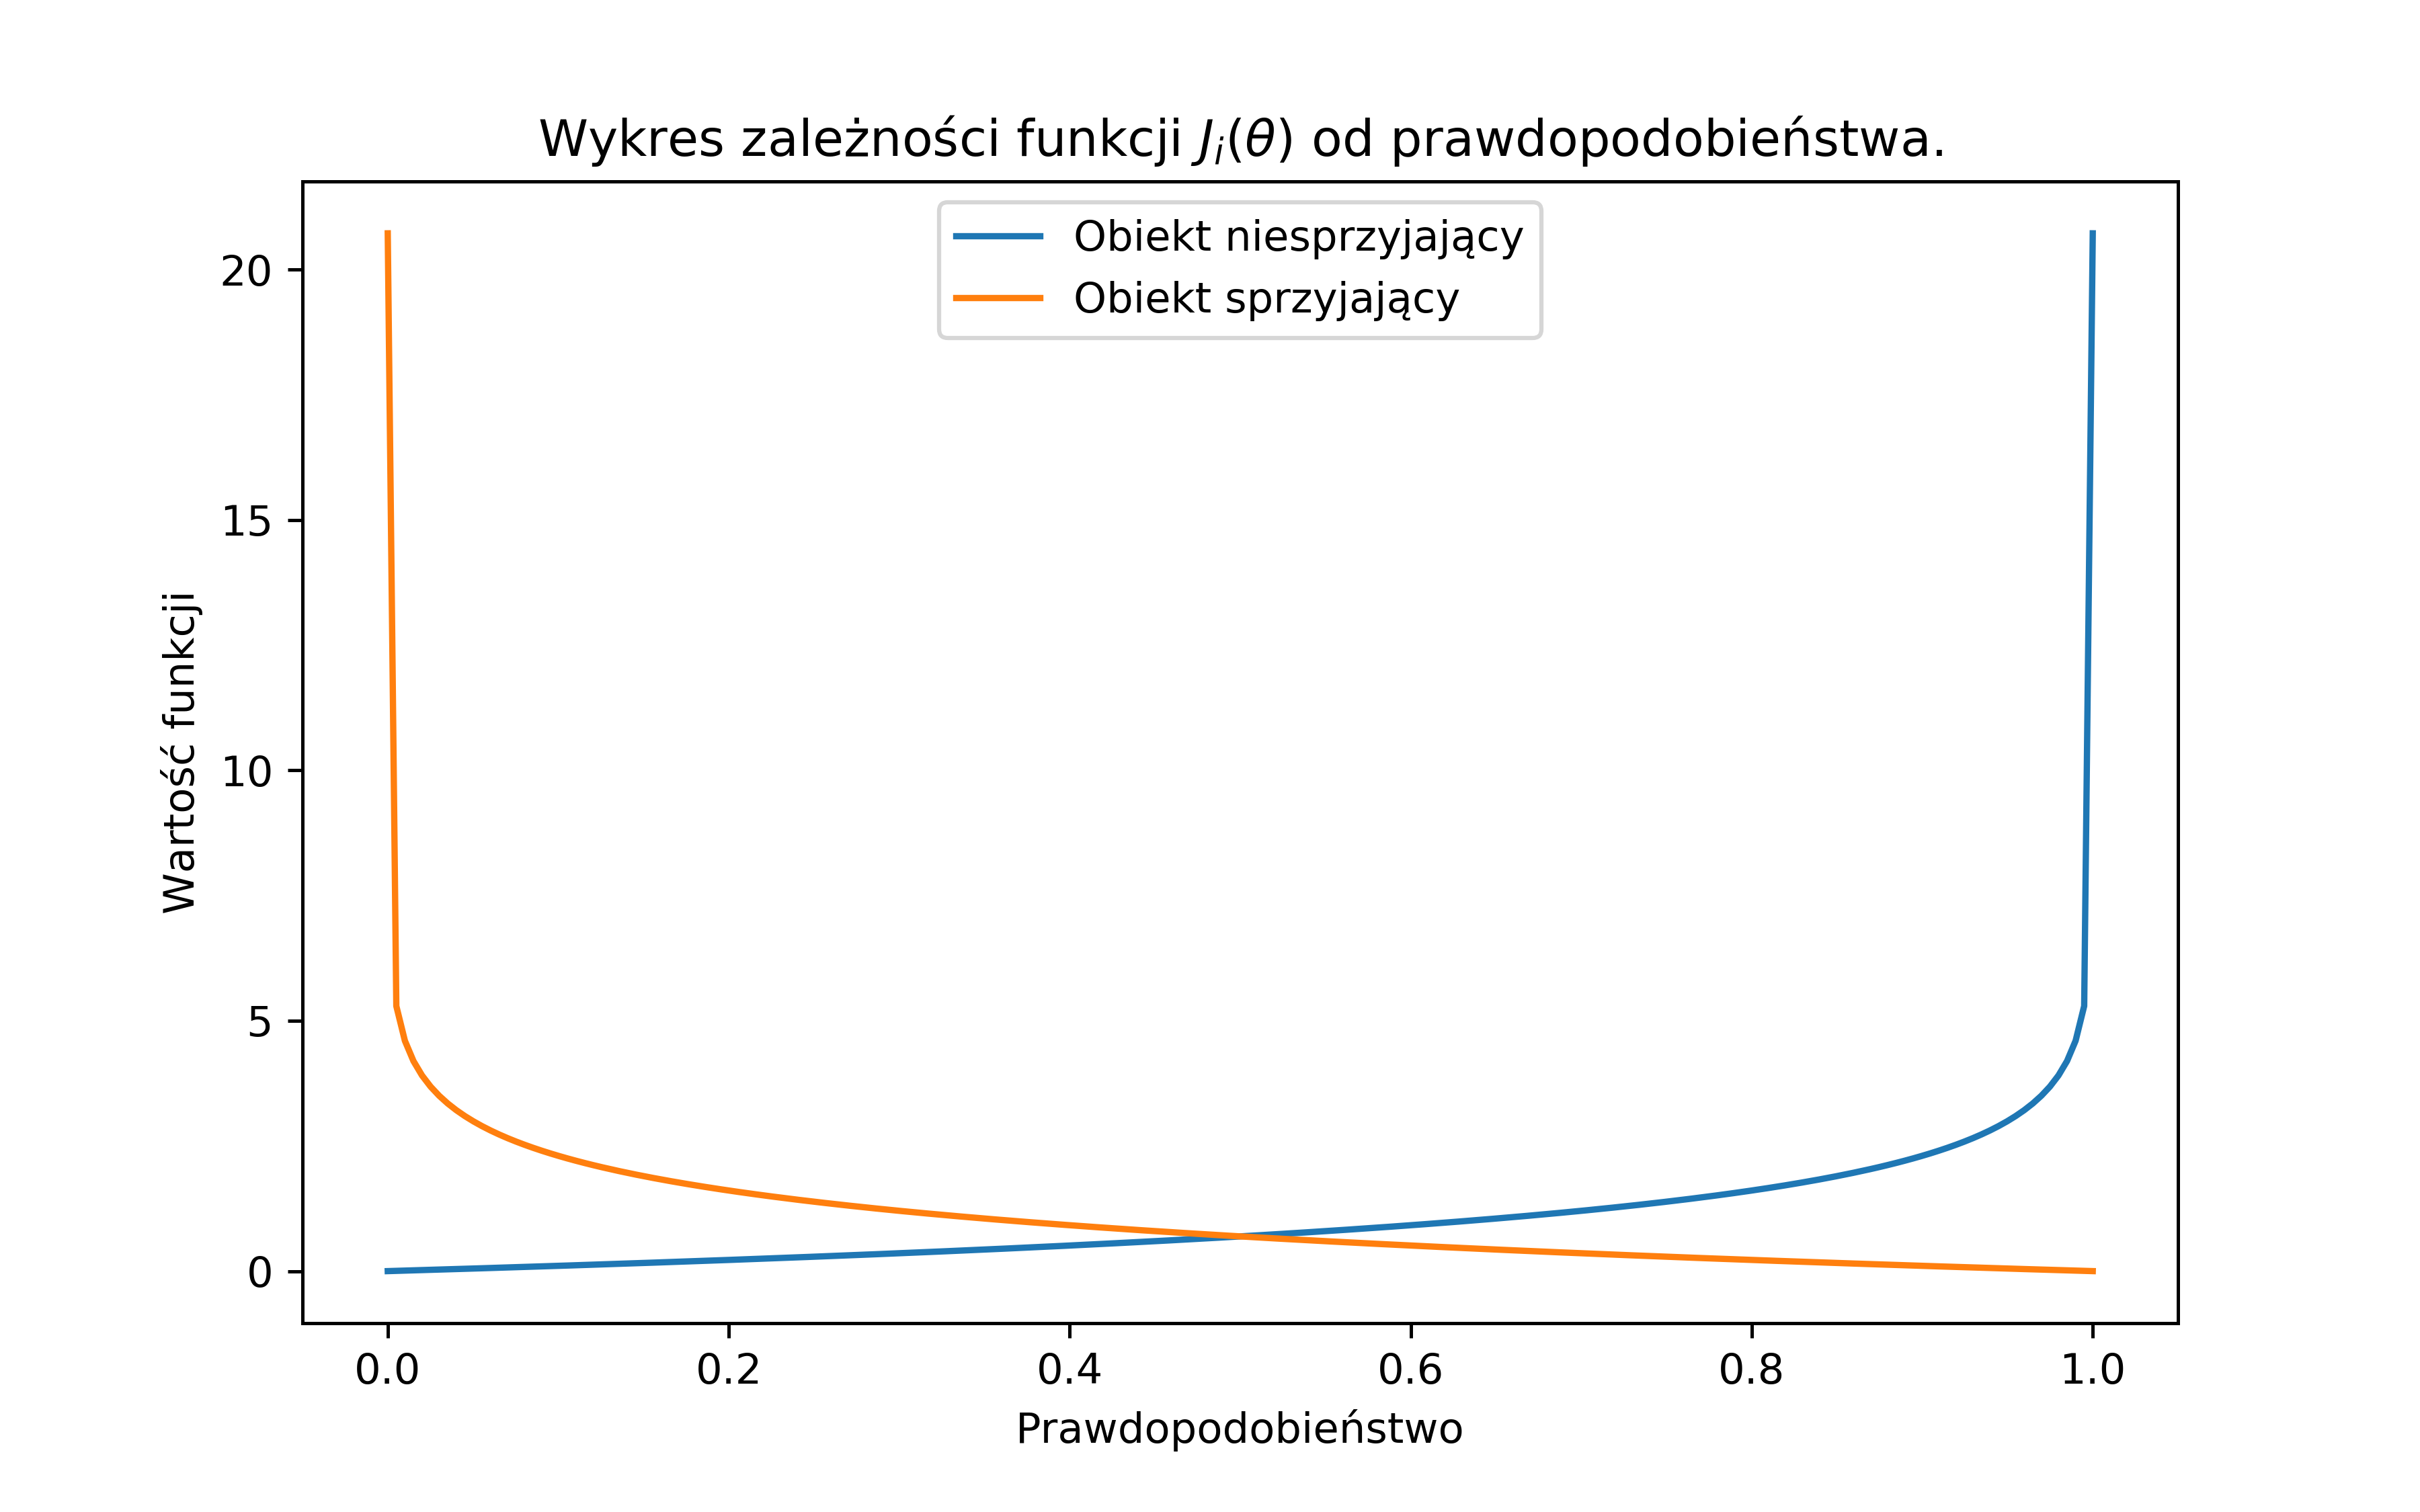
\includegraphics[width=\linewidth]{images/cross_entropy.png}
	\caption{Wykres zależności funkcji $J_i(\theta)$ od prawdopodobieństwa predykcji danej obserwacji. Kolor niebieski przedstawia wykres dla próbki o prawdziwej klasie pozytywnej, natomiast kolor pomarańczowy dla negatywnej. Źródło: Opracowanie własne.}
	\label{fig:cross-entropy-plot}
\end{figure}

W~literaturze dotyczącej uczenia maszynowego zamiast funkcji logarytmu wiarogodności $l(\theta | \es, \ytrue)$ definiuje się funkcję straty $J(\theta)$, która w~przypadku regresji logistycznej przyjmuje postać
$$ J(\theta) =  - l(\theta | \es, \ytrue) = \sum_{i=1}^N J_i(\theta) \text{.}$$
W~celu lepszego zrozumienia funkcji straty regresji logistycznej przyjrzymy się bliżej własnościom funkcji $J_i(\theta)$. Wykres \ref{fig:cross-entropy-plot} przedstawia przyjmowane wartości funkcji $J_i(\theta)$ w~zależności od estymowanego prawdopodobieństwa $\htx$. Kolorem niebieskim jest oznaczony przebieg funkcji dla obiektu niesprzyjającego, a pomarańczowym dla sprzyjającego. Możemy zauważyć, że dla obu rodzajów obiektów, funkcja $J_i(\theta)$ jest odbiciem funkcji dla przeciwnego obiektu względem prostej pionowej dla prawdopodobieństwa równego $0.5$. Oznacza to, że ten klasyfikator przykłada taką samą wagę dla obu rodzajów błędów. Ponadto rozważając następujące granice dla $y_i=0$
$$ \lim\limits_{\htx\to 0^+} -\log(1-\htx) = 0 \text{,}$$
$$ \lim\limits_{\htx\to 1^-} -\log(1-\htx) = \infty $$
oraz dla $y_i=1$
$$ \lim\limits_{\htx\to 0^+} -\log(\htx) = \infty \text{,}$$
$$ \lim\limits_{\htx\to 1^-} -\log(\htx) = 0 $$
otrzymujemy, że koszt klasyfikacji dla pojedynczej obserwacji przyjmuje w przybliżeniu następujące wartości
$$
J_i(\theta) \approx \left\{
\begin{array}{rl}
0, &\mbox{jeżeli $\htx \approx y_i$}, \\
\infty, &\mbox{jeżeli $1 - \htx \approx y_i$}.
\end{array}{}
\right.
$$
Powyższe wyprowadzenie oznacza, że w przypadku prawidłowego zaklasyfikowania danej obserwacji funkcja przyjmuje wartość bliską zeru, natomiast w przypadku pomyłki nieskończoności. Stąd możemy wywnioskować, że koszty popełnienia bądź niepopełnienia błędu są następujące:
$$ C^{(i)}_{1,1} = C^{(i)}_{0,0} \approx 0 \text{,}$$
$$ C^{(i)}_{1,0} = C^{(i)}_{0,1} \approx \infty \text{.}$$
Jest to wynik, który nie oddaje charakteru nierówności kosztu popełniania różnych błędów, stąd powstaje motywacja, aby zmodyfikować podaną funkcję i stworzyć regresję logistyczną, która będzie w stanie modyfikować koszty poszczególnych klasyfikacji. Przykład takiego modelu jest omówiony w~sekcji \ref{cslr}.

\subsection{Drzewo decyzyjne}
\label{drzewo}
Drzewo decyzyjne to nieparametryczny model uczenia nadzorowanego, który jest wykorzystywany do regresji oraz klasyfikacji. Jego celem jest nauczenie się na podstawie dostępnych danych prostych reguł decyzyjnych. Do jego największych zalet należy łatwość interpretacji otrzymanych wyników oraz niewielka ilość niezbędnych przygotowań danych, ponieważ między innymi nie wymagają one normalizacji, skalowania lub transformacji zmiennych kategorycznych.

Poniżej opiszemy trzy rodzaje najpopularniejszych algorytmów, które są odpowiedzialne za proces uczenia drzew.
\begin{itemize}
	\item ID3 (Iterative Dichotomiser 3) -- algorytm pozwala na tworzenie drzew decyzyjnych, które w poszczególnych węzłach mogą mieć więcej niż dwa podziały. Działa jedynie dla zmiennych kategorycznych. Drzewo rośnie do maksymalnego rozmiaru, a następnie jest przycinane;
	\item C4.5 -- następca ID3, który znosi restrykcję używania tylko kategorycznych atrybutów poprzez dyskretyzację zmiennych ciągłych. Nauczone drzewo zamieniane jest w zestaw reguł, które są szeregowane względem poprawy skuteczności. Przycinanie w tym wypadku polega na usuwanie reguł, które nie poprawiają wyniku modelu;
	\item CART (z angielskiego \textit{Classification and Regression Tree}) -- bardzo podobny algorytm do C4.5, który umożliwia tworzenie drzew regresyjnych (w poprzednich algorytmach mamy do czynienia jedynie z zadaniami klasyfikacyjnymi) oraz nie tworzy zestawu reguł. Konstruuje on binarne drzewa, które do podziału używa atrybutu oraz progu odcięcia maksymalizującego przyrost informacji.
\end{itemize}
Warto zaznaczyć, że implementacja w bibliotece \textit{sklearn} w Pythonie wykorzystuje zmodyfikowaną wersję algorytmu CART, który nie obsługuje zmiennych kategorycznych. Poniżej prezentujemy teorię matematyczną stojącą za implementacją tego algorytmu \cite{sklearn_api}.

Niech $\ku$ będzie zbiorem obserwacji dla danego węzła $m$. Ponadto niech podział będzie reprezentowany przez parę $\theta = (j, t_m)$, gdzie $j$ odpowiada $j$-temu atrybutowi wektora $\iks_i$, natomiast $t_m$ to warunek podziału danych na podzbiory $\ku_l$ oraz $\ku_r$, gdzie
$$ \ku_l (\theta) = \{ \iks_i : \iks_i \in \ku \land x^{(j)}_i \leq t_m \} \text{,} $$
$$ \ku_r (\theta) = \ku \setminus \ku_l(\theta) \text{.} $$
Czystość danego węzła jest wyznaczana w następujący sposób
$$ G(\ku, \theta) = \frac{|\ku^l (\theta)|}{|\ku|} I(\ku_l (\theta)) + \frac{|\ku^r (\theta)|}{|\ku|} I(\ku_r (\theta)) \text{,}$$
gdzie $I(\cdot)$ może być dowolną funkcją miary zanieczyszczenia. Ostatecznie w~danym węźle wybierany jest ten podział, który minimalizuje funkcję czystości
$$ \theta^* = \argmin_\theta G(\ku, \theta) \text{.}$$
Dalej następuje rekurencyjny podział na podzbiory wyznaczonego $\ku_l (\theta^*)$ i niezależnie $\ku_r (\theta^*)$. Algorytm działa do osiągnięcia maksymalnej głębokości drzewa. W zależności od implementacji oraz preferencji użytkownika po zakończeniu działania algorytmu wykonuje się przycinanie drzewa. Jest to metoda, która w ogólności polega na usuwaniu nadmiarowych węzłów, które mogą powodować zbyt dokładne dopasowanie do danych. Ponadto ostatnie podzbiory, które pozostały na końcu drzewa, nazywamy liśćmi. 
W~momencie predykcji wykorzystujemy utworzone podziały, aby dla zadanej obserwacji znaleźć odpowiedni liść. Następnie model zwraca prawdopodobieństwo należenia do poszczególnych klas, które jest równe procentowi próbek z~danej klasy w~danych treningowych w~znalezionym liściu.


W~zależności od rodzaju problemu, wykorzystujemy różne miary zanieczyszczenia \cite{sklearn_api}. Dla zadań klasyfikacyjnych są to
\begin{itemize}
	\item Misclassification: $I_m(\ku) = 1 - \max(p(\ku), 1 - p(\ku))$,
	\item Entropy: $I_e(\ku) = -p(\ku) \log_2 p(\ku) - (1 - p(\ku)) \log_2(1 - p(\ku))$,
	\item Gini: $I_g(\ku) = 2p(\ku)(1 - p(\ku))$,
\end{itemize}{}
a dla zadań regresyjnych
\begin{itemize}
	\item $ \displaystyle I_{mse}(\ku) = \frac{1}{|\ku|} \sum_{i \in \ku} (y_i - q(\ku))^2$,
	\item $ \displaystyle I_{mae}(\ku) = \frac{1}{|\ku|} \sum_{i \in \ku} |y_i - q(\ku)|$,
\end{itemize}
gdzie:
$$ p(\ku) = \frac{| \{ \iks_i : \iks_i \in \ku \land y_i = 1 \}|}{|\ku|} \text{,} $$
$$ q(\ku) = \frac{\sum_{i \in \ku} y_i}{|\ku|} \text{.} $$

\subsection{Las losowy}
Las losowy oraz algorytm XGBoost są przedstawicielami szerokiej klasy modeli typu \textit{ensemble}. Głównym celem tej metodologii jest wprowadzenie losowych perturbacji do zbioru treningowego, w~celu utworzenia różnych klasyfikatorów bazowych, których wspólne predykcje będą lepsze niż każdego z modeli bazowych osobno. Ponadto istnieją trzy główne powody, dlaczego te metody działają znacznie lepiej niż pojedyncze modele:
\begin{itemize}
	\item Statystyczny -- w przypadku, gdy mamy do czynienia z małym zbiorem danych, istnieje możliwość stworzenia kilku bardzo dobryh klasyfikatorów, które na zbiorze treningowym mają taką samą skuteczność. W przypadku dodatkowego zbioru testowego istnieje szansa wybrania nieoptymalnego;
	\item Obliczeniowy -- większość algorytmów polega na optymalizacji numerycznej, która może zatrzymać się w minimum lokalnym. Dzięki zastosowaniu kilku modeli uzyskujemy szansę przeszukania większej części przestrzeni parametrów modeli;
	\item Reprezentacyjny -- często funkcja $f$ reprezentująca prawdziwy model jest bardzo skomplikowana i niemożliwe jest przedstawienie jej za pomocą jednego modelu. Wykorzystując złożenie kilku modeli bazowych, mamy szansę lepiej przybliżać prawdziwą funkcję $f$.
\end{itemize}

W celu utworzenia $T$ klasyfikatorów bazowych, należy ze zbioru treningowego $\es$ wybrać $S_j$ dla $j=1,2,\dots,T$ losowych podzbiorów obserwacji, które wykorzystamy do uczenia. W tym celu wykorzystuje się następujące procedury losowania.

\begin{itemize}
	\item Wklejanie (\textit{ang. Pasting}) -- Polega na niezależnym losowaniu $K < N$ próbek ze zbioru $\es$ bez powtórzeń. Najczęściej wykorzystywana jest na bardzo dużych zbiorów danych, gdzie zasoby obliczeniowe są ograniczone i nie jest możliwe wczytanie wszystkich danych do pamięci komputera. Ponadto dzięki możliwości wykorzystania obliczeń równoległych skraca się czas tworzenia całego modelu. Próbki mogą być losowane z rozkładu jednostajnego, bądź wykorzystując metody biorące pod uwagę ważność poszczególnych obserwacji \cite{Pasting}.
	\item Workowanie (\textit{ang. Bagging}) -- Polega na niezależnym losowaniu $K \leq N$ próbek ze zbioru $\es$ z powtórzeniami. Najczęściej jest wykorzystywany w przypadku małych zbiorów danych, kiedy chcemy wykorzystać maksymalnie dużą ilość obserwacji, lecz także wprowadzić losowość do kolejnych klasyfikatorów bazowych.
	\item Losowe podprzestrzenie (\textit{ang. Random Subspaces}) -- Metoda polegająca na wybraniu do każdego klasyfikatora bazowego wszystkich obserwacji, lecz losuje się tylko część atrybutów opisujące dane. Głównym celem tego zabiegu jest poprawa skuteczności poprzez zwiększenie różnorodności klasyfikatorów bazowych \cite{Random_Subspace}.
	\item Losowe łaty (\textit{ang. Random Patches}) -- Procedura łącząca metodę wklejania z losowymi podprzestrzeniami. Jej celem jest połączenie zalet obu metod i ostatecznie poprawienie skuteczności modelu z~jednoczesną optymalizacją wykorzystywanego czasu oraz pamięci \cite{Random_Patches}.
\end{itemize}
Na rysunku \ref{fig:sampling_plot} na stronie \pageref{fig:sampling_plot} schematycznie przedstawiono wyżej omówione zasady działania poszczególnych procedur losowania. Należy zwrócić uwagę zarówno na powtarzające się lub nie numery wierszy, jak i~na kolory kolumny symbolizujące odpowiednie zmienne z~oryginalnego zbioru danych.
\begin{figure}[h]
	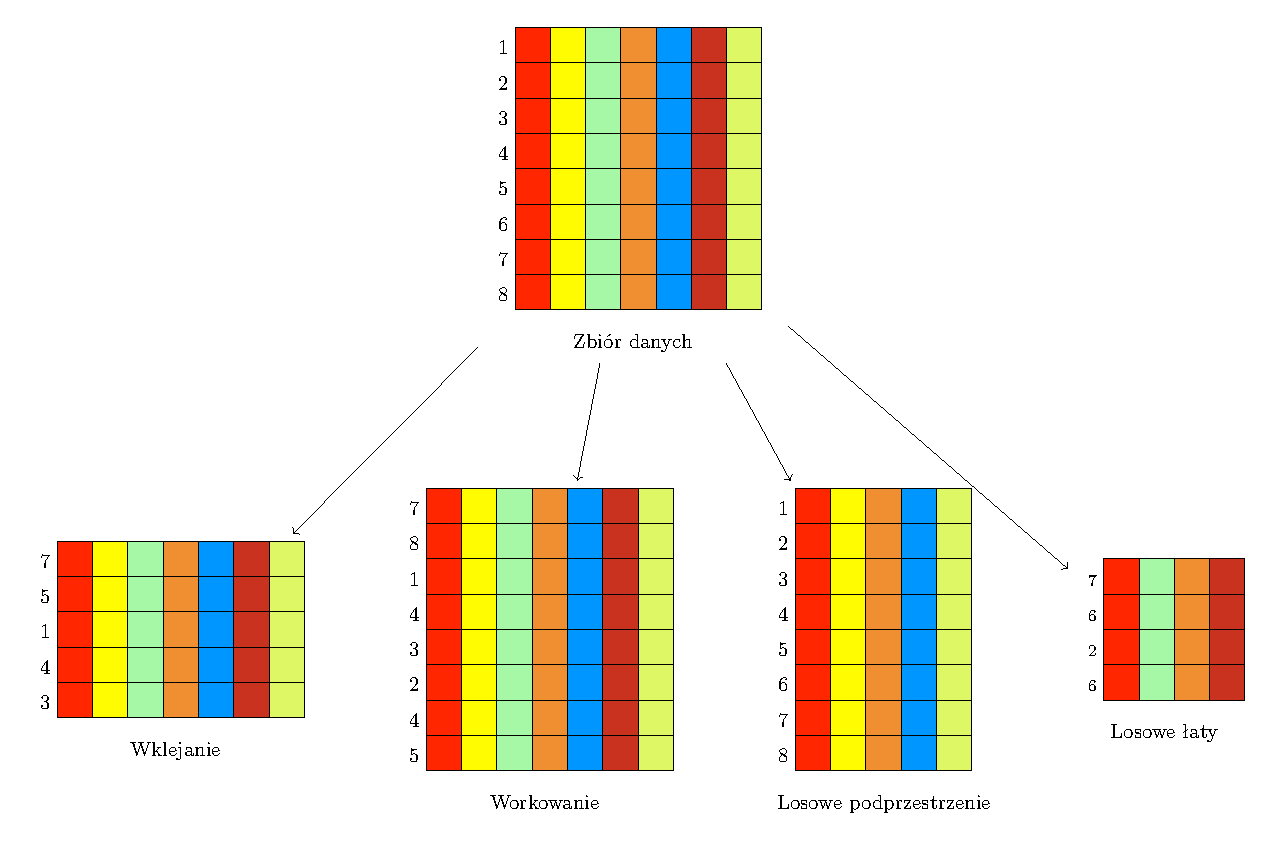
\includegraphics[width=\linewidth]{plots/sampling_plot.pdf}
	\caption{Schemat działania procedur losowania. Źródło: Opracowanie własne.}
	\label{fig:sampling_plot}
\end{figure}

Warto zauważyć, że mimo tego, że powyższe metody były oryginalnie tworzone z~myślą o~wykorzystaniu drzewa decyzyjnego jako klasyfikatora bazowego, to nic nie stoi na przeszkodzie, aby wykorzystać inny model. Ten fakt został użyty na przykład w~pracy A.~Bahnsena \cite{alej2015ensemble}, gdzie wykorzystując omawiane w sekcji \ref{csdt} drzewa decyzyjne wrażliwe na koszt, stworzono lasy losowe wrażliwe na koszt.

Procedura tworzenia lasu losowego jest podzielona na dwie fazy \cite{Random_Forest}. Pierwsza z~nich wykorzystuje workowanie do wygenerowania odpowiednich próbek dla klasyfikatorów bazowych. Następnie trenujemy zmodyfikowane drzewa decyzyjne, które na etapie tworzenia każdego kolejnego węzła w drzewie losują podzbiór zmiennych do wyboru podziału. Finalnie podczas predykcji każdy model dokonuje klasyfikacji i ostatecznym wynikiem modelu jest klasyfikacja większość głosów. Nie jest to jedyna możliwość agregowania wyników, przykładowo wykorzystywana w~bibliotece \textit{sklearn} w~języku programowania Python, implementacja uśrednia wyniki prawdopodobieństwa z~każdego klasyfikatora \cite{sklearn_api}.

\subsection{XGBoost}
W~ogólności proces trenowania modeli w~uczeniu maszynowym polega na znalezieniu najlepszych parametrów modelu $\theta$, które najlepiej pasują do danych treningowych ze zbioru $\es$ i~ich prawdziwych wartości $\ytrue$. W~celu dokonania tego procesu definiujemy funkcję celu (\textit{ang. objective}), którą w ogólnej postaci możemy zapisać jako
\begin{equation}
	\label{obj-general}
	\text{Obj}(\theta) = J(\theta) + \Omega(\theta) \text{,}
\end{equation}
gdzie $J(\theta)$ to funkcja straty, a $\Omega(\theta)$ to wyraz odpowiadający za regularyzację, która nakłada odpowiednie kary na współczynniki modelu, aby zapobiec zbytniemu dopasowaniu do danych. Za funkcję straty najczęściej przyjmujemy w przypadku zadań regresyjnych błąd średniokwadratowy
$$ J(\theta) = \frac{1}{N} \sum_{i=1}^{N} (y_i - \hat{y_i})^2 \text{,}$$
gdzie $\hat{y_i}$ to predykcja modelu dla $i$-tej obserwacji i~zależy ona od parametrów modelu $\theta$, lub w przypadku zadań klasyfikacyjnych entropię krzyżową daną równaniem \eqref{c-e}.

Algorytm XGBoost (\textit{ang. Extreme Gradient Boosting}) to model, który w~iteracyjny sposób tworzy kolejne drzewa decyzyjne typu CART (patrz sekcja \ref{drzewo}). Na potrzeby algorytmu drzewa są zmodyfikowane i~na liściu nie zawierają samej decyzji binarnej, lecz przypisują liczbę rzeczywistą, która daje znacznie bogatszą reprezentację \cite{xgboost}. Podobnie jak w przypadku lasu losowego wykorzystujemy wiele klasyfikatorów bazowych, a następnie dzięki wykorzystywanej reprezentacji możemy zapisać predykcję $i$-tej obserwacji jako
$$ \hat{y_i} = \sum_{k=1}^K f_k(\iks_i) \text{,} \quad f_k \in \ef \text{,} $$
gdzie $K$ oznacza liczbę drzew decyzyjnych, $f_k$ funkcje z przestrzeni $\ef$ wszystkich możliwych drzew CART. Warto zaznaczyć, że w~przypadku zagadnienia regresyjnego predykcja $y_i$ jest bezpośrednim wynikiem, natomiast dla problemów klasyfikacyjnych wykorzystuje się funkcję sigmoidalną (podobnie jak w regresji logistycznej) w~celu zamiany wartości liczby rzeczywistej na predykcję z~przedziału $[0,1]$.

Korzystając z ogólnej postaci funkcji celu danej równaniem \eqref{obj-general} na stronie \pageref{obj-general} funkcja $\text{Obj}(\theta)$, którą będziemy optymalizować, przyjmuje następującą postać
$$ \text{Obj}(\theta) = \sum_{i=1}^{N} l(y_i, \hat{y_i}) + \sum_{k=1}^{K} \Omega(f_k) \text{,} $$
gdzie $l(y_i, \hat{y_i})$ to funkcja straty, przykładowo błąd średniokwadratowy lub entropia krzyżowa, a $\Omega(f_k)$ to regularyzacja nałożona na drzewo $f_k$, przykładowo ograniczenie głębokości drzewa.

Uczenie drzew decyzyjnych jest znacznie trudniejszym zadaniem niż standardowe zagadnienia optymalizacyjne, gdyż w tym przypadku nie jesteśmy w stanie wprost policzyć gradientu i~wyliczyć kolejnych wartości współczynników. Zamiast tego użyjemy uczenia addytywnego, które w~każdym kroku iteracji naprawia błędne klasyfikacje z~poprzedniego kroku oraz tworzy kolejne drzewo. Przez $\yht{t}$ będziemy oznaczać predykcję dla $i$-tej obserwacji w~kroku $t$. Zatem możemy zapisać kolejne predykcje w następujący sposób:
$$ \yht{0} = 0 \text{,}$$
$$ \yht{1} = f_1(x_i)  = \yht{0} + f_1(x_i) \text{,}$$
$$ \yht{2} = f_1(x_i) + f_2(x_i) = \yht{1} + f_2(x_i) \text{,}$$
$$ ... $$
$$ \yht{t} = \sum_{k=1}^{t} f_k(x_i) = \yht{t-1} + f_t(x_i) \text{.}$$
Podczas każdego z~kroków iteracji będziemy chcieli minimalizować odpowiednią funkcję celu, która w~tym przypadku ma postać
$$ \text{Obj}^{(t)}(\theta) = \sum_{i=1}^{N} l(y_i, \yht{t}) + \sum_{k=1}^{t} \Omega(f_k) \text{.} $$
Wykorzystując powyższe wzory, otrzymujemy następujące wyrażenie
$$ \text{Obj}^{(t)}(\theta) = \sum_{i=1}^{N} l(y_i, \yht{t-1} + f_t(x_i)) + \Omega(f_t) + \text{const.}$$
Korzystając z rozwinięcia szeregu Taylora dla funkcji straty, otrzymujemy ogólny wzór:
$$ \text{Obj}^{(t)}(\theta) = \sum_{i=1}^{N} \left[ l(y_i, \yht{t-1}) + g_i f_t(x_i) + \frac{1}{2} h_i f_t^2(x_i) \right] + \Omega(f_t) + \text{const. ,} $$
gdzie:
$$ g_i = \partial_{\yht{t-1}} l(y_i, \yht{t-1}) \text{,} $$
$$ h_i = \partial^2_{\yht{t-1}} l(y_i, \yht{t-1}) \text{.}$$
Następnie po redukcji stałych, które są nieistotne z punktu widzenia optymalizacji, otrzymujemy
$$ \sum_{i=1}^{N} [g_i f_t(x_i) + \frac{1}{2} h_i f_t(x_i)] + \Omega(f_t) \text{.}$$
Zauważmy, że nigdzie bezpośrednio nie korzystaliśmy z postaci funkcji straty, zatem w ten sposób jesteśmy w stanie zbudować model optymalizujący dowolną dwukrotnie różniczkowalną funkcję ciągłą. Taka uniwersalność powoduje, że algorytm ten znajduje zastosowanie w wielu zadniach z zakresu uczenia maszynowego, jak i innych problemów optymalizacyjnych.

\section{Klasyfikacja wrażliwa na koszt}
Metody klasyfikacji wrażliwej na koszt (\textit{ang. Cost Dependent Classification})  są przykładem pierwszego rodzaju modeli wrażliwych na koszt. W przypadku tych metod trening zawierający informację o koszcie odbywa się dopiero po etapie stworzenia modelu zwracającego prawdopodobieństwa. Cały proces jest przedstawiony na rysunku \ref{cdc} na stronie \pageref{cdc}. Górna część diagramu przedstawia standardowy proces uczenia modelu predykcyjnego, natomiast dolna część reprezentuje schemat dokonywania predykcji. W~celu wyznaczenia decyzji klasyfikatora najpierw estymujemy prawdopodobieństwa dla zbioru testowego, a~następnie wykorzystując otrzymane wartości oraz koszt klasyfikacji, dokonujemy ostatecznej decyzji. Warto wspomnieć, że w~celu dokonania treningu modelu klasyfikacji wrażliwej na koszt potrzebujemy dodatkowego podzbioru danych, który nie był wykorzystywany do uczenia standardowego modelu.
\begin{figure}[h]
	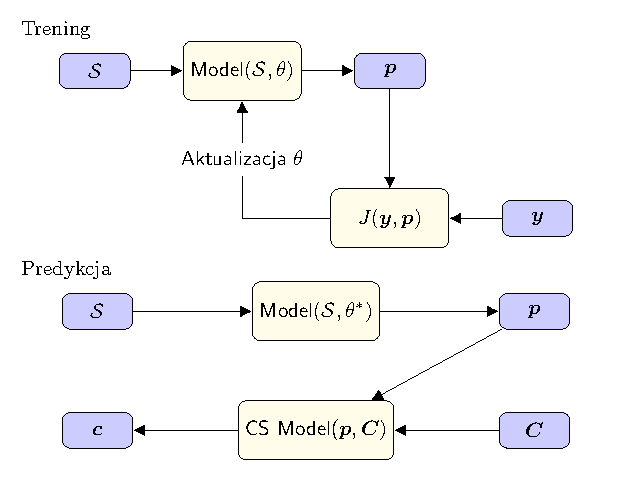
\includegraphics[width=\linewidth]{plots/cost_sensitive_classification.pdf}
	\caption{Schemat przedstawiający proces uczenia klasyfikatora wrażliwego na koszt. Źródło: Opracowanie własne na podstawie artykułu \cite{RMoser}.}
	\label{cdc}
\end{figure}
\subsection{Optymalizacja progu}
Metoda optymalizacji progu (TO, z angielskiego \textit{threshold optimization}) jest popularną metodą wyznaczania odpowiedniego progu prawdopodobieństwa, powyżej którego wszystkie obserwacje oznaczamy jako pozytywnie zaklasyfikowane, a poniżej negatywnie. Może być ona wykorzystywana nie tylko do problemów wrażliwych na koszt, lecz do dowolnie zdefiniowanego zagadnienia, w którym potrzebne są zero-jedynkowe predykcje. Jej sformułowanie wygląda następująco
$$ t^{*} = \argmax_{t \in [0,1]} f(\ytrue, \boldsymbol{c}) \text{,} $$
gdzie:
\begin{itemize}
	\item $f(\cdot, \cdot) $ -- funkcja miary skuteczności modelu, która jako argumenty przyjmuje wektor prawdziwych wartości klasyfikacji oraz wektor binarnych predykcji, np. dokładność,
	\item $\boldsymbol{c} = (\mathbbm{1}_{\{p_i > t\}})_{i=1}^n $ -- wektor binarnych klasyfikacji modelu,
	\item $ \text{t} $ -- wartość progu decyzyjnego.
\end{itemize}{}
W naszym przypadku funkcją $f$ będzie funkcja oszczędności (\ref{oszczednosci}). Innymi słowy, będziemy szukać takiego progu decyzyjnego, który zmaksymalizuje wartość oszczędności.

\subsection{Minimalizacja ryzyka bayesowskiego}
\label{bmr}
Minimalizacja ryzyka bayesowskiego (BMR, z angielskiego \textit{Bayesian Minimum Risk}) to model decyzyjny, którego celem jest zmierzenie oraz porównanie wartości prawdopodobieństw wystąpienia pewnych zdarzeń i kosztów związanych z podjęciem określonych decyzji  \cite{CSCCFD}. Polega na przypisaniu odpowiedniej wartości reprezentującej ryzyko zaklasyfikowania danej obserwacji jako pozytywnej lub negatywnej, które definiujemy w następujący sposób
$$ R(c_i = 1|\iks_{i}) = L(c_i = 1|y_i = 1)P(y_i = 1|\iks_{i}) + L(c_i = 1|y_i = 0)P(y_i = 0|\iks_{i}) \text{,}$$
$$ R(c_i = 0|\iks_{i}) = L(c_i = 0|y_i = 1)P(y_i = 1|\iks_{i}) + L(c_i = 0|y_i = 0)P(y_i = 0|\iks_{i}) \text{,}$$
gdzie
\begin{itemize}
	\item $P(y_i = 1|\iks_{i})$, $P(y_i = 0|\iks_{i})$ -- oznaczają estymowane przez model prawdopodobieństwa zaklasyfikowania obserwacji jako odpowiednio pozytywna oraz negatywna klasa i~$P(y_i = 0|\iks_{i}) = 1 - P(y_i = 1|\iks_{i})$,
	\item $L(c_i = j|y_i = k)$ oraz $j,k \in \{0, 1\}$ -- funkcja kosztu, która określa stratę, którą poniesiemy w zależności od wyniku poprawności klasyfikacji.
\end{itemize}{}
Zauważmy, że powyższe równania możemy zapisać jako
$$ R(c_i = c|\iks_{i}) = L(c_i = c|y_i = 1)P(y_i = 1|\iks_{i}) + L(c_i = c|y_i = 0)P(y_i = 0|\iks_{i})\text{.} $$
Rozważając przypadek binarny, możemy bez straty ogólności przyjąć, że
$$ L(c_i = j|y_i = k) = C_{j, k}^{(i)} \text{,}$$
zatem wzór na ryzyko przyjmuje postać
$$ R(c_i = c|\iks_{i}) = C_{c, 1}^{(i)}P(y_i = 1|\iks_{i}) + C_{c, 0}^{(i)}P(y_i = 0|\iks_{i})\text{.} $$
Ponadto warto zauważyć, że traktując $y_i$ jako zmienną losową możemy zapisać ryzyko klasyfikacji danej obserwacji jako
$$ R(c_i = c|\iks_{i}) = E[C_{c, y_i}^{(i)} | \iks_{i}] \text{.}$$

Decyzja dotycząca danej obserwacji jest opisana następującą nierównością
$$ c_i = 1 \Leftrightarrow R(c_i = 1|\iks_{i}) \leq R(c_i = 0|\iks_{i})$$
i oznacza ona, że klasyfikujemy dany przykład jako pozytywny, jeżeli ryzyko takiej decyzji jest mniejsze niż zaklasyfikowania danej obserwacji jako negatywną. 
Po przeprowadzaniu odpowiednich przekształceń algebraicznych (wyprowadzone w~dodatku \ref{bmr-proof}) oraz zakładając, że 
$$ C_{0, 1}^{(i)} - C_{1, 1}^{(i)} - C_{0, 0}^{(i)} + C_{1, 1}^{(i)} > 0 \text{,}$$ 
otrzymujemy następujący wzór na klasyfikację przykładu jako pozytywny
$$ c_i = 1 \Leftrightarrow P(c_i = 1|\iks_{i}) \ge \frac{C^{(i)}_{1,0} - C^{(i)}_{0,0}}{C^{(i)}_{0,1} - C^{(i)}_{1,1} - C^{(i)}_{0,0} + C^{(i)}_{1,0}} \text{.}$$

\section{Trening wrażliwy na koszt}
Drugą podgrupą metod wrażliwych na koszt jest trening wrażliwy na koszt (\textit{ang.~Cost Sensitive Trainig}). Metody te już na etapie treningu modelu biorą pod uwagę koszt związany z~klasyfikacją danej obserwacji. Schemat uczenia modelu jest przedstawiony na wykresie \ref{cst} na stronie \pageref{cst}. Algorytm jako wejście otrzymuje zbiór danych treningowych, następnie dokonuje predykcji i~na bazie prawdziwych odpowiedzi oraz kosztów wyznaczana jest skuteczność modelu. W następnej kolejności aktualizowane są wagi, a cały proces jest iteracyjnie powtarzany, aż do momentu osiągnięcia zadanego kryterium stopu. Predykcja w~tym przypadku następuje w~standardowy sposób.
\begin{figure}[h]
	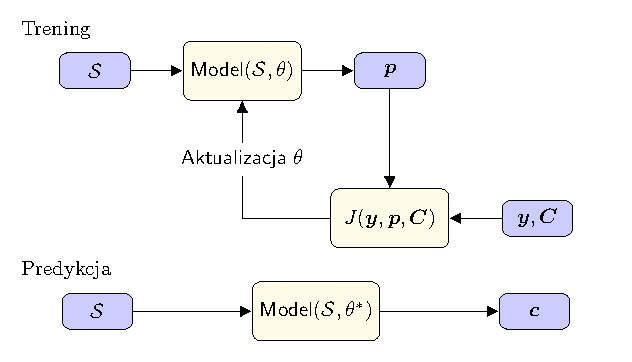
\includegraphics[width=\linewidth]{plots/cost_sensitive_training.pdf}
	\caption{Schemat przedstawiający proces uczenia modelu wrażliwego na koszt. Źródło: Opracowanie własne na podstawie artykułu \cite{RMoser}.}
	\label{cst}
\end{figure}	

\subsection{Regresja logistyczna wrażliwa na koszt}
\label{cslr}
Pierwszym modelem, który zostanie omówiony, jest regresja logistyczna wrażliwa na koszt. Kontynuując rozważania z podrozdziału \ref{reg-log}, chcemy, aby funkcja straty standradowego modelu przyjmowała następujące wartości, które odpowiadają wartościom z~macierzy kosztu
$$
J^c_i(\theta)=\left\{
\begin{array}{rl}
C^{(i)}_{1,1}, &\mbox{jeżeli $y_i = 1$ i $\htx \approx 1$}, \\
C^{(i)}_{0,0}, &\mbox{jeżeli $y_i = 0$ i $\htx \approx 0$}, \\
C^{(i)}_{1,0}, &\mbox{jeżeli $y_i = 0$ i $\htx \approx 1$}, \\
C^{(i)}_{0,1}, &\mbox{jeżeli $y_i = 1$ i $\htx \approx 0$}.
\end{array}
\right.
$$
Przykładową funkcją, która zachowuje się w następujący sposób, jest

$$ J^c_i(\theta) = y_i \Big( \htx C^{(i)}_{1,1} + (1 - \htx)C^{(i)}_{0,1} \Big) + (1-y_i) \Big( \htx C^{(i)}_{1,0} + (1 - \htx)C^{(i)}_{0,0} \Big) \text{.} $$


\begin{figure}[h]
	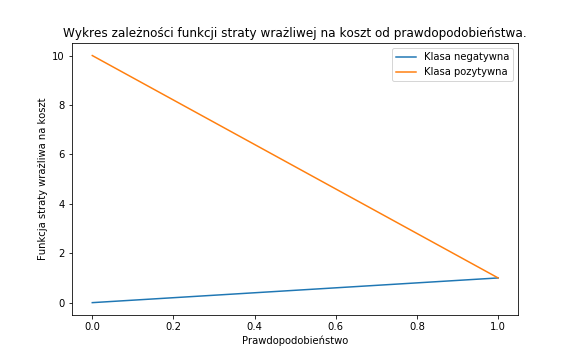
\includegraphics[width=\linewidth]{images/cost_sensitive_ce.png}
	\caption{Wykres zależności wrażliwej na koszt funkcji straty od prawdopodobieństwa predykcji danej obserwacji. Kolor niebieski przedstawia wykres dla próbki o prawdziwej klasie pozytywnej, natomiast kolor pomarańczowy dla negatywnej. Wykres dla przykładowych wartości: $C^{(i)}_{1,1} = 1 \text{, } C^{(i)}_{0,1} = 10 \text{, } C^{(i)}_{1,0} = 1 \text{, } C^{(i)}_{0,0} = 0$. Źródło: Opracowanie własne.}
	\label{fig:cost-sensitive-loss-function}
\end{figure}

Wykres funkcji $J^c_i(\theta)$ jest przedstawiony na wykresie \ref{fig:cost-sensitive-loss-function} na stronie \pageref{fig:cost-sensitive-loss-function}. Kolor niebieski przedstawia wykres dla próbki o prawdziwej klasie pozytywnej, natomiast kolor pomarańczowy dla negatywnej. Możemy zauważyć pożądaną przez nas asymetrię popełniania błędów oraz osiąganie przez funkcję odpowiednich wartości w granicach prawdopodobieństwa równego $0$ oraz $1$.

Ostatecznie funkcją, którą będziemy minimalizować, jest 
$$ J^c(\theta) = \sum_{i=1}^{N} J^c_i(\theta) \text{.} $$
Podobnie jak w przypadku standardowej regresji logistycznej, wykorzystując algorytm optymalizujący, szukamy optymalnych współczynników modelu.

\subsection{Drzewo decyzyjne wrażliwe na koszt}
\label{csdt}
Analogicznie jak w~przypadku regresji logistycznej należy wprowadzić kosztu klasyfikacji danej próbki do procesu powstawania drzewa decyzyjnego. Naturalnym miejscem do uzależnienia modelu od kosztu klasyfikacji jest moment podziału danego węzła. Do tej pory wszystkie miary zanieczyszczenia skupiały się na możliwe najlepszym rozróżnieniu próbek w kontekście minimalizacji liczby błędów klasyfikacji. Zamiast tego, w~przypadku metody wrażliwej na koszt, naszym celem jest minimalizacja kosztu. W~tym celu definiujemy następującą miarę zanieczyszczenia
$$ I_c(\ku) = \text{Koszt bazowy}(\ytrue^{\ku}, \boldsymbol{C}^{\ku}) \text{,}$$
gdzie górny indeks $\ku$ oznacza odpowiedni podzbiór obserwacji, które wybieramy do wektora $\ytrue$ oraz $\boldsymbol{C}$. Intuicja stojąca za takim sformułowaniem jest następująca. Klasyfikujemy wszystkie przypadki w rozważanym podziale jako pozytywne, następnie jako negatywne i~sprawdzamy, która z decyzji miała mniejszy sumaryczny koszt. W~momencie predykcji ostateczny werdykt, który może być tylko binarny, zależy od tego, która klasyfikacja minimalizuje sumaryczny koszt na liściu.

\chapter{Eksperyment}
W~celu porównania klasycznych oraz wrażliwych na koszt metod predykcyjnych przeprowadzono eksperyment na danych dotyczących detekcji oszustw na kartach płatniczych. Istotą doświadczenia było sprawdzenie, czy metody wrażliwe na koszt dają lepsze rezultaty niż standardowe modele. Jeżeli tak, to czy dzieje się tak dla każdej z metod, czy tylko dla niektórych. Ponadto, jeżeli nastąpi poprawa wyników względem oszczędności, to czy dzieje się to kosztem skuteczności w~sensie standardowych miar. 

Pierwsza część rozdziału dotyczy omówienia zawartości oraz pochodzenia zbioru danych. Dalej zostanie przedstawiona metodologia przeprowadzania eksperymentu. Rozważania zostaną zakończone omówieniem otrzymanych wyników oraz wyciągniętych wniosków.

\section{Dane}
Do eksperymentu został wykorzystany zbiór danych \emph{Credit Card Fraud Detection}\footnote{Źródło: \url{https://www.kaggle.com/mlg-ulb/creditcardfraud}}, który składa się z~transakcji zawartych europejskimi kartami kredytowymi w~ciągu dwóch dni we wrześniu 2013 roku. Dane były zebrane na potrzeby badań naukowych grupy Worldline and the Machine Learning Group\footnote{Strona grupy Worldline and the Machine Learning Group: \url{http://mlg.ulb.ac.be}} z~Université Libre de Bruxelles. Zbiór zawiera 284,807 transakcji w tym zaledwie 492 oszustwa. Tabela składa się z~30 kolumn, w~tym 28 z~nich to zanonimizowane zmienne numeryczne, które były wcześniej poddane transformacji PCA (\textit{ang. Principal Component Analysis}), a pozostałe dwie kolumny to informacje dotyczące godziny oraz kwoty transakcji. Ponadto wśród danych nie ma brakujących wartości. Podczas modelowania pominiemy zmienną czasową, ponieważ sama w sobie nie zawiera ona istotnej informacji, a tworzenie znaczących zmiennych nie jest istotą przeprowadzanego eksperymentu. 

Mimo tego, że dane zostały poddane anonimizacji, to na podstawie artykułu A.~Bahnsena możemy domyślać się, z~jakimi zmiennymi mieliśmy do czynienia przed transformacjami \cite{CSCCFD}. Podczas procesu dokonywania transakcji standardowo zbierane są: 
\begin{itemize}
	\item[--] data dokonania transakcji, 
	\item[--] numer konta,
	\item[--] numer karty,
	\item[--] typ transakcji (płatność internetowa, płatność stacjonarna, wypłata z bankomatu),
	\item[--] kwota, 
	\item[--] ID beneficjenta transakcji,
	\item[--] grupa beneficjenta transakcji (przykładowo linie lotnicze, hotel, wypożyczalnia samochodów itp.), 
	\item[--] kraj dokonania transakcji,
	\item[--] kraj zamieszkania właściciela karty,
	\item[--] typ karty (przykładowo VISA, MasterCard itp.),
	\item[--] wiek klienta, 
 	\item[--] płeć klienta,
	\item[--] bank klienta,
	\item[--] historyczna informacja czy dana transakcja była oszustwem.
\end{itemize}
\noindent Na podstawie wymienionych informacji tworzy się agregaty czasowe bazujące na historii, których celem jest zebranie informacji dotyczących nawyków zakupowych danego klienta~\cite{bahnsen_presentation}. Stworzenie takiej zmiennej rozpoczyna się od zgrupowania transakcji z~pewnego odcinka czasowego najpierw według id klienta lub karty kredytowej, a~następnie przez typ transakcji, beneficjenta transakcji, kategorię beneficjenta lub kraj. Proces kończy się agregacją powstałych grup poprzez zsumowanie wartości tych transakcji lub zliczenie ich ilości. Przykładowymi zmiennymi, które powstają w tym procesie, są ilość transakcji dla tego samego klienta w~ciągu ostatnich 6 godzin, średnia wartość transakcji w sklepach spożywczych dla danej karty kredytowej z~ostatniego tygodnia. 

Na podstawie wiedzy dotyczącej modelowania detekcji oszustw z~artykułu A. Bahnsena~\cite{alej2015ensemble} w~tabeli \ref{tab:macierz-kosztu-eksperyment} na stronie \pageref{tab:macierz-kosztu-eksperyment} definiujemy wartości kosztu dla tego eksperymentu. Poniżej krótkie objaśnienie.
\begin{itemize}
	\item Wartość $C_a = 1$ to stały koszt administracyjny podjęcia sprawy przez analityka, który sprawdza, czy dana obserwacja jest faktycznie oszustwem, niezależnie od tego, jaki był jego ostateczny werdykt.
	\item $\text{Amt}_i$ to wartość transakcji, jaką utracimy w~przypadku niewskazanie fałszywej transakcji jako oszustwa.
	\item Zerowa wartość kosztu dla normalnej obserwacji, która była prawidłowo wskazana, pochodzi z~braku konieczności podjęcia inwestygacji oraz strat z tego wynikających.
\end{itemize} 

\begin{table}[h]
	\begin{center}
		\begin{tabular}{c|c|c}
			\multirow{2}{4em}{} & Stan pozytywny & Stan negatywny \\
			& $y_i = 1$            & $y_i = 0$ \\
			\hline
			Predykcja pozytywna & \multirow{2}{8em}{\centering $C^{(i)}_{1,1} = \text{C}_{\text{a}} = 1$} & \multirow{2}{8em}{\centering $C^{(i)}_{1,0} = \text{C}_{\text{a}} = 1$} \\
			$c_i = 1$         &                    &                    \\
			\hline
			Predykcja negatywna & \multirow{2}{8em}{\centering $C^{(i)}_{0,1} = \text{Amt}_{\text{i}}$} & \multirow{2}{8em}{\centering $C^{(i)}_{0,0} = 0$} \\
			$c_i = 0$         &                    &                    \\
		\end{tabular}
	\end{center}
	\caption{Macierz kosztu eksperymentu.}
	\label{tab:macierz-kosztu-eksperyment}
\end{table}

\section{Opis eksperymentu}
Inspiracja do eksperymentu pochodzi z pracy A. Bahnsena dotyczącej porównania metod wrażliwych na koszt dla pięciu rzeczywistych zbiorów danych~\cite{alej2015ensemble}. Dane pochodzą z~czterech różnych dziedzin zastosowań: detekcja oszustw na kartach kredytowych, prognoza rezygnacji, ryzyko kredytowe oraz marketing bezpośredni. Celem pracy było porównanie standardowych metod oraz metod wrażliwych na koszt na przykładzie innego zbioru danych. Do eksperymentu wykorzystano regresję logistyczną, drzewo decyzyjne, las losowy, XGBoost oraz drzewo decyzyjne wrażliwe na koszt. Ponadto standardowe modele zostały rozszerzone metodą optymalizacji progu (TO) oraz minimalizacji ryzyka bayesowskiego (BMR). Modyfikacją, w~stosunku do oryginalnego eksperymentu, było użycie algorytmu XGBoost, który dotychczas w~wielu standardowych zastosowaniach uzyskiwał znacznie lepsze wyniki od reszty modeli uczenia maszynowego.

W~celu przeprowadzenia eksperymentu zbiór danych został pięćdziesięciokrotnie podzielony w~proporcjach 50:17:33 na odpowiednio zbiór treningowy, walidacyjny oraz testowy. Losowanie nowych podziałów zbioru miało na celu zmniejszenie ryzyka, że wynik będzie zależny od wylosowanej próbki. Ponadto wykorzystano tę technikę zamiast standardowej warstwowej walidacji krzyżowej (\textit{ang. Stratified Cross Validation}) z~uwagi na zbyt małą próbkę testową, która powstaje w~przypadku wykorzystania walidacji krzyżowej. Następnie wytrenowano wszystkie modele standardowe oraz drzewo decyzyjne wrażliwe na koszt na zbiorze treningowym. Dla modelu XGBoost wykorzystano zbiór walidacyjny do procesu wczesnego zatrzymywania (\textit{ang. Early Stopping}), natomiast dla modeli BMR oraz TO wykorzystano ten zbiór jako treningowy. Następnie dla wszystkich modeli dokonano predykcji na zbiorze testowym i~zmierzono skuteczność typowań, wykorzystując miarę oszczędności oraz $F_1$ Score. Ostatecznie wyniki z~wszystkich pięćdziesięciu prób zostały uśrednione oraz obliczono wartości odchyleń standardowych.

Do implementacji skryptów wykorzystano język programowania Python wraz z~bibliotekami \textit{costcla}, \textit{sklearn}, \textit{pandas}, \textit{numpy}, \textit{matplotlib} oraz język programowania BASH. Kody źródłowe programu można znaleźć w~dodatku \ref{scripts}.

\section{Wyniki}

Wyniki eksperymentu dla miary oszczędności są zaprezentowane na wykresie \ref{fig:results-savings} na stronie \pageref{fig:results-savings}. Szare, niebieskie oraz czerwone słupki oznaczają dla pierwszych czterech modeli: regresji logistycznej (LogisticRegression), drzewa decyzyjnego (DecisionTree), lasu losowego (RandomForest) oraz XGBoosta, odpowiednio model standardowy, model optymalizacji progu oraz model wykorzystujący minimalizację ryzyka bayesowskiego. Dla modelu drzewa decyzyjnego wrażliwego na koszt (CS Decision Tree) posiadamy jedynie szary słupek, ponieważ model ten sam w sobie jest już wrażliwy na koszt i~nie potrzebuje dodatkowych modyfikacji. 

Możemy zauważyć, że wśród standardowych modeli oraz drzewa decyzyjnego wrażliwego na koszt najmniejszy wynik oszczędności uzyskała regresja logistyczna a~największy las losowy, XGBoost oraz drzewo decyzyjne wrażliwe na koszt. Dodatkowo zwraca uwagę fakt, że wrażliwa na koszt wersja drzewa decyzyjnego przyniosła lepsze rezultaty niż standardowy model. W~przypadku, gdy weźmiemy pod uwagę rozszerzone wersje modeli standardowych o~klasyfikację wrażliwą na koszt, to zdecydowanie najlepszym modelem okazał się XGBoost w~połączeniu z~minimalizacją ryzyka bayesowskiego. Warto zauważyć, że w~przypadku optymalizacji progu wartość oszczędności jest większa lub równa niż wynik uzyskany przez standardowy model. Dla minimalizacji ryzyka bayesowskiego zachodzi podobna sytuacja, gdzie w~każdym przypadku wyniki są lepsze. Ponadto średnia wartość oszczędności modelu BMR w~obrębie każdego z modeli standardowych jest najwyższa. Podsumowując, w~przypadku tego eksperymentu, gdyby najważniejsza byłaby dla nas wartość oszczędności, to najlepszym wyborem byłby algorytm XGBoost z dodatkowym modelem minimalizacji ryzyka bayesowskiego. Co więcej, w~każdym z~przypadków, model wrażliwy na koszt poprawia wynik oszczędności.

\begin{figure}
	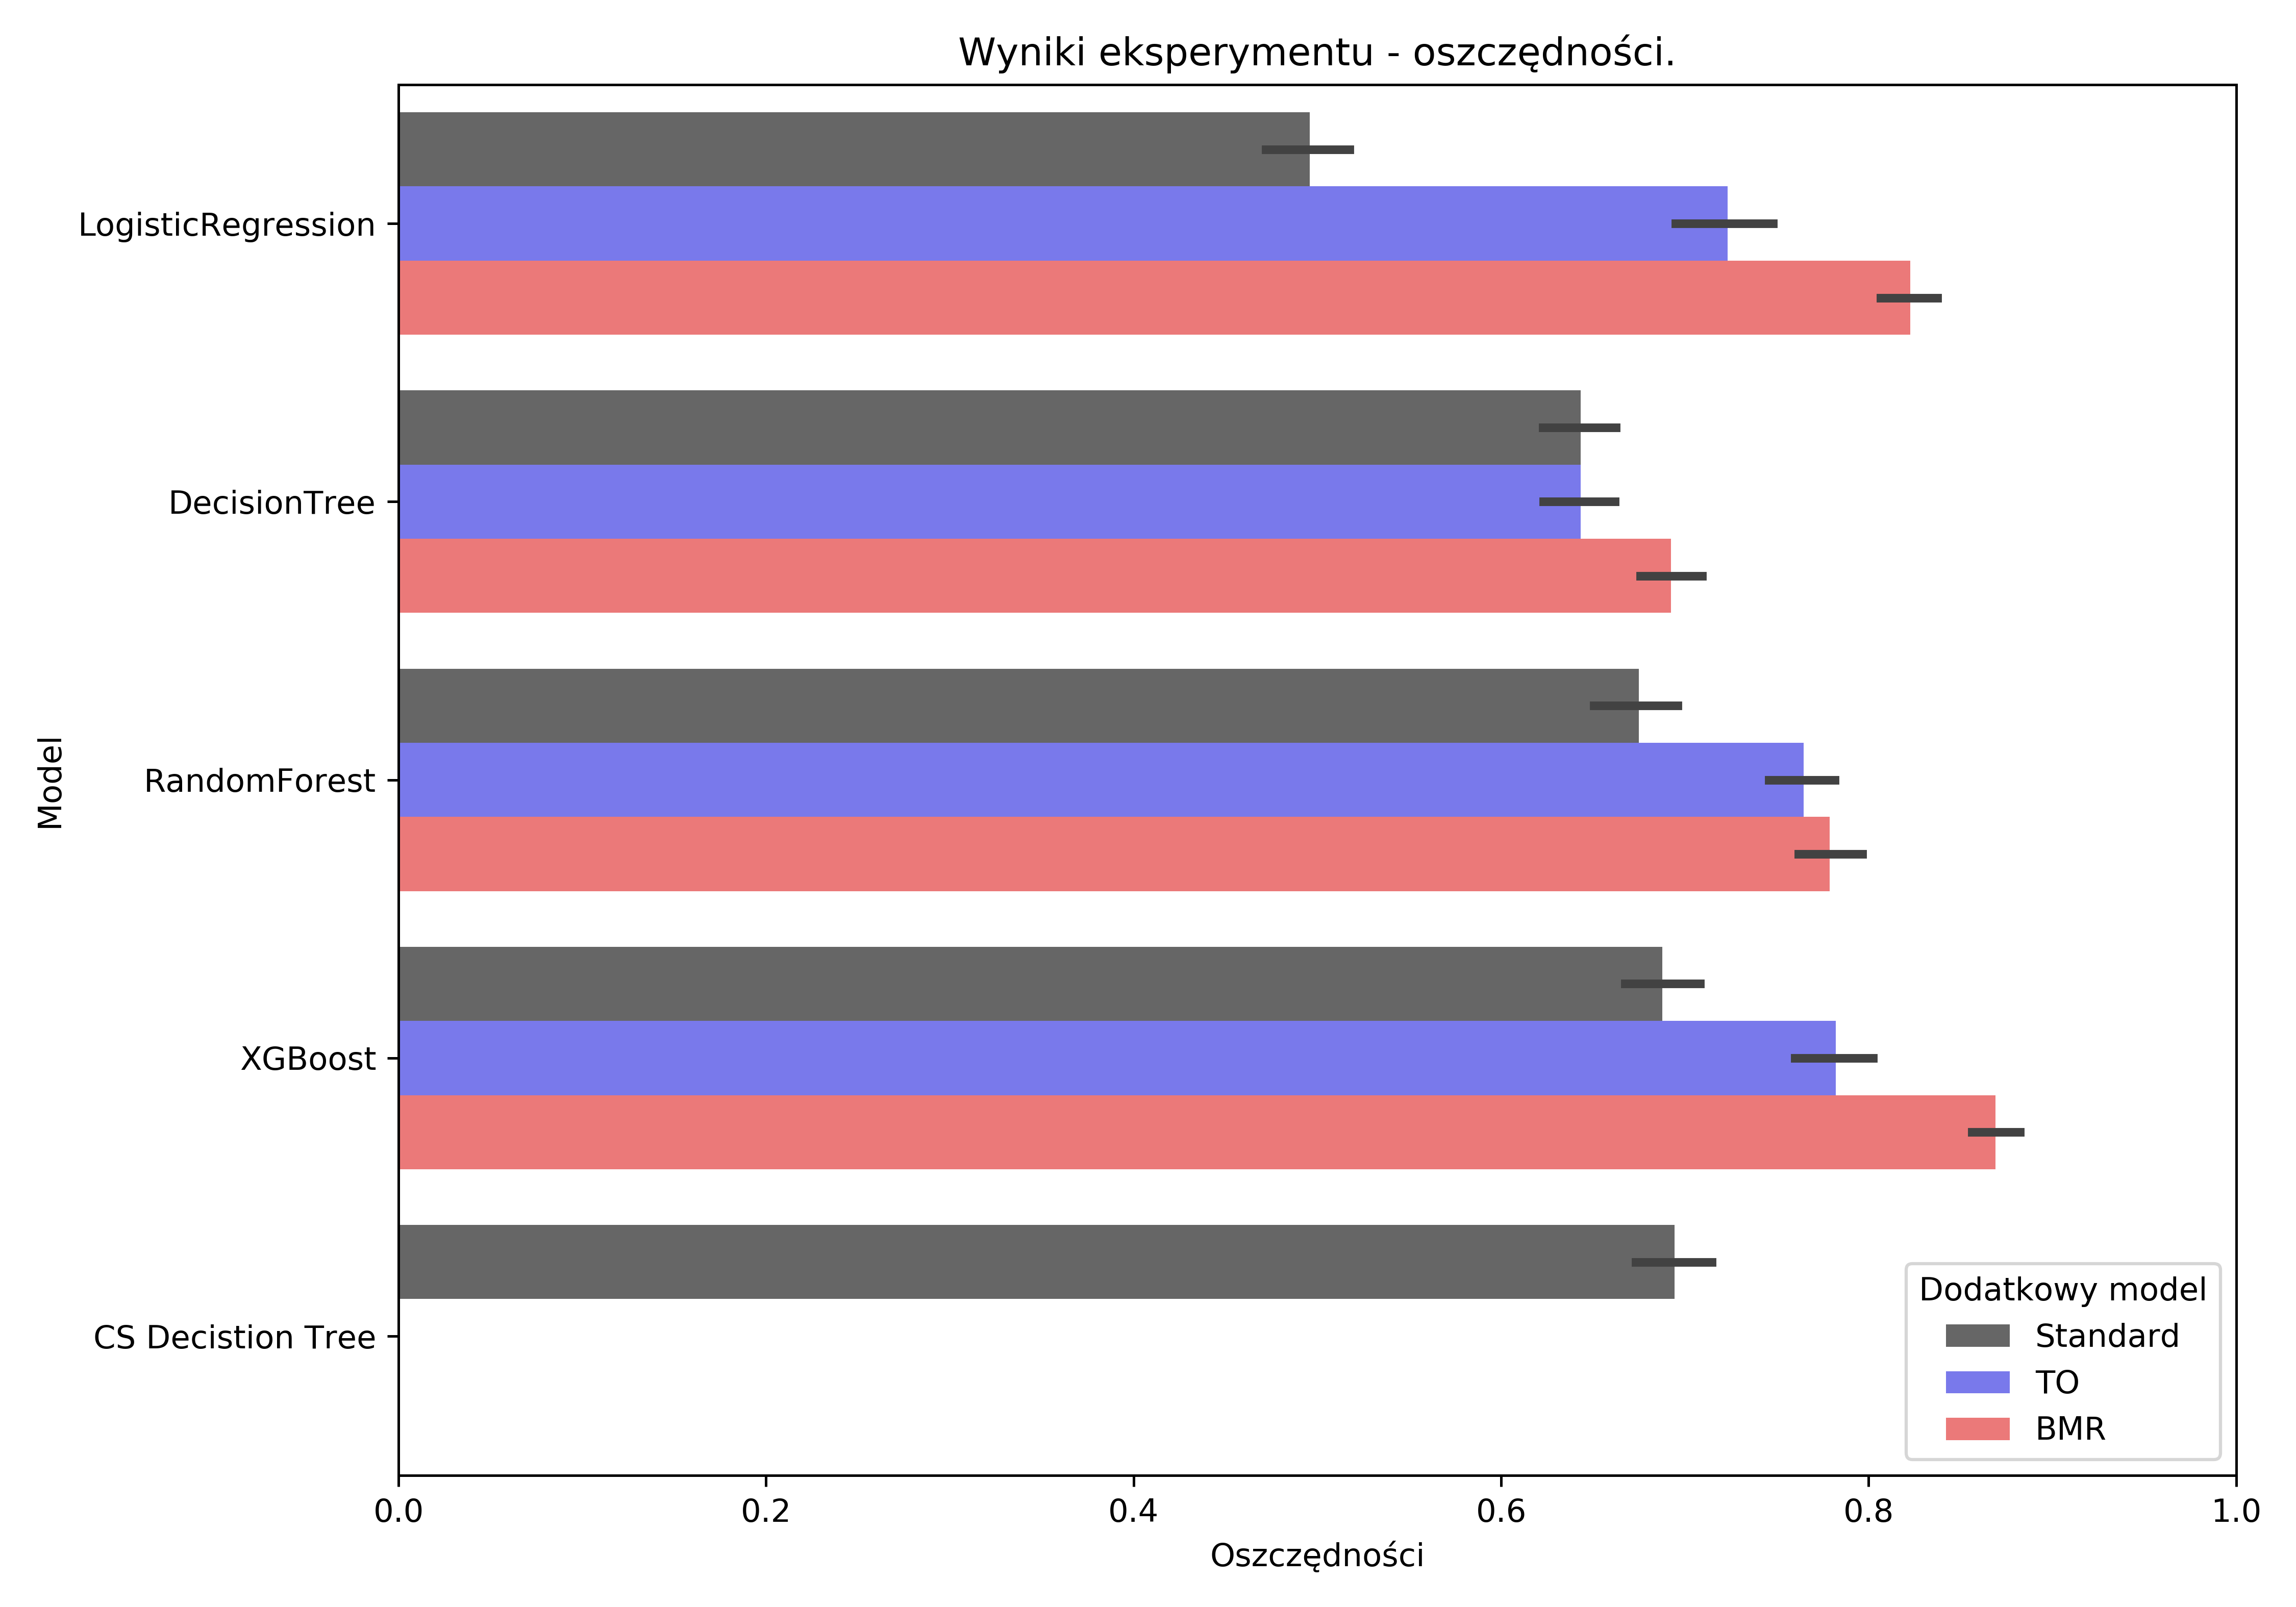
\includegraphics[width=\linewidth]{images/100_config1-Savings.png}
	\caption{Wyniki eksperymentu dla miary skuteczności oszczędności. Szare, niebieskie oraz czerwone słupki oznaczają dla pierwszych czterech modeli: regresji logistycznej (LogisticRegression), drzewa decyzyjnego (DecisionTree), lasu losowego (RandomForest) oraz XGBoosta, odpowiednio model standardowy, model optymalizacji progu oraz model wykorzystujący minimalizację ryzyka bayesowskiego. Dla modelu drzewa decyzyjnego wrażliwego na koszt (CS Decision Tree) mamy jedynie jedną wartość. Wysokość słupka reprezentuje wartość średnią z 50 powtórzeń, a długość dołączonej kreski oznacza $\pm$ wartość odchylenia standardowego w odpowiednią stronę. Źródło: Opracowanie własne.}
	\label{fig:results-savings}
\end{figure}

W~celu porównania zmiany skuteczności modeli względem standardowych miar przeanalizujemy wyniki eksperymentu dla $F_1$ Score, które są zaprezentowane na wykresie~\ref{fig:results-f1} na stronie \pageref{fig:results-savings}. Oznaczenia są analogiczne jak do wykresu dotyczącego oszczędności. Możemy zauważyć, że dla standardowych wersji modeli w przypadku tej miary skuteczności najlepsze rezultaty osiągnął las losowy oraz XGBoost. Dodatkowo model drzewa decyzyjnego wrażliwego na koszt uzyskał w~tym wypadku gorsze rezultaty niż standradowa wersja. W~przypadku klasyfikacji wrażliwej na koszt modele optymalizacji progu prawie zawsze pogarszały wyniki (z wyjątkiem drzewa decyzyjnego, gdzie wynik był taki sam jak bez modelu), a dla minimalizacji ryzyka bayesowskiego wynik zawsze był gorszy od standardowej wersji modelu. Intuicyjnie jest to zrozumiały rezultat, ponieważ nasz model przestał zwracać uwagę na transakcje, które miały małą wartość, nawet jeżeli przypadek ten był łatwy do wykrycia, a profilaktycznie zaczął sprawdzać duże transakcje, które mogły mieć nawet małe prawdopodobieństwa bycia oszustwem. W~związku z tym modele zaczęły oszczędzać więcej pieniędzy kosztem ogólnej skuteczności modelu, przez to zwracają większą ilości fałszywie pozytywnych klasyfikacji. 

\begin{figure}[h]
	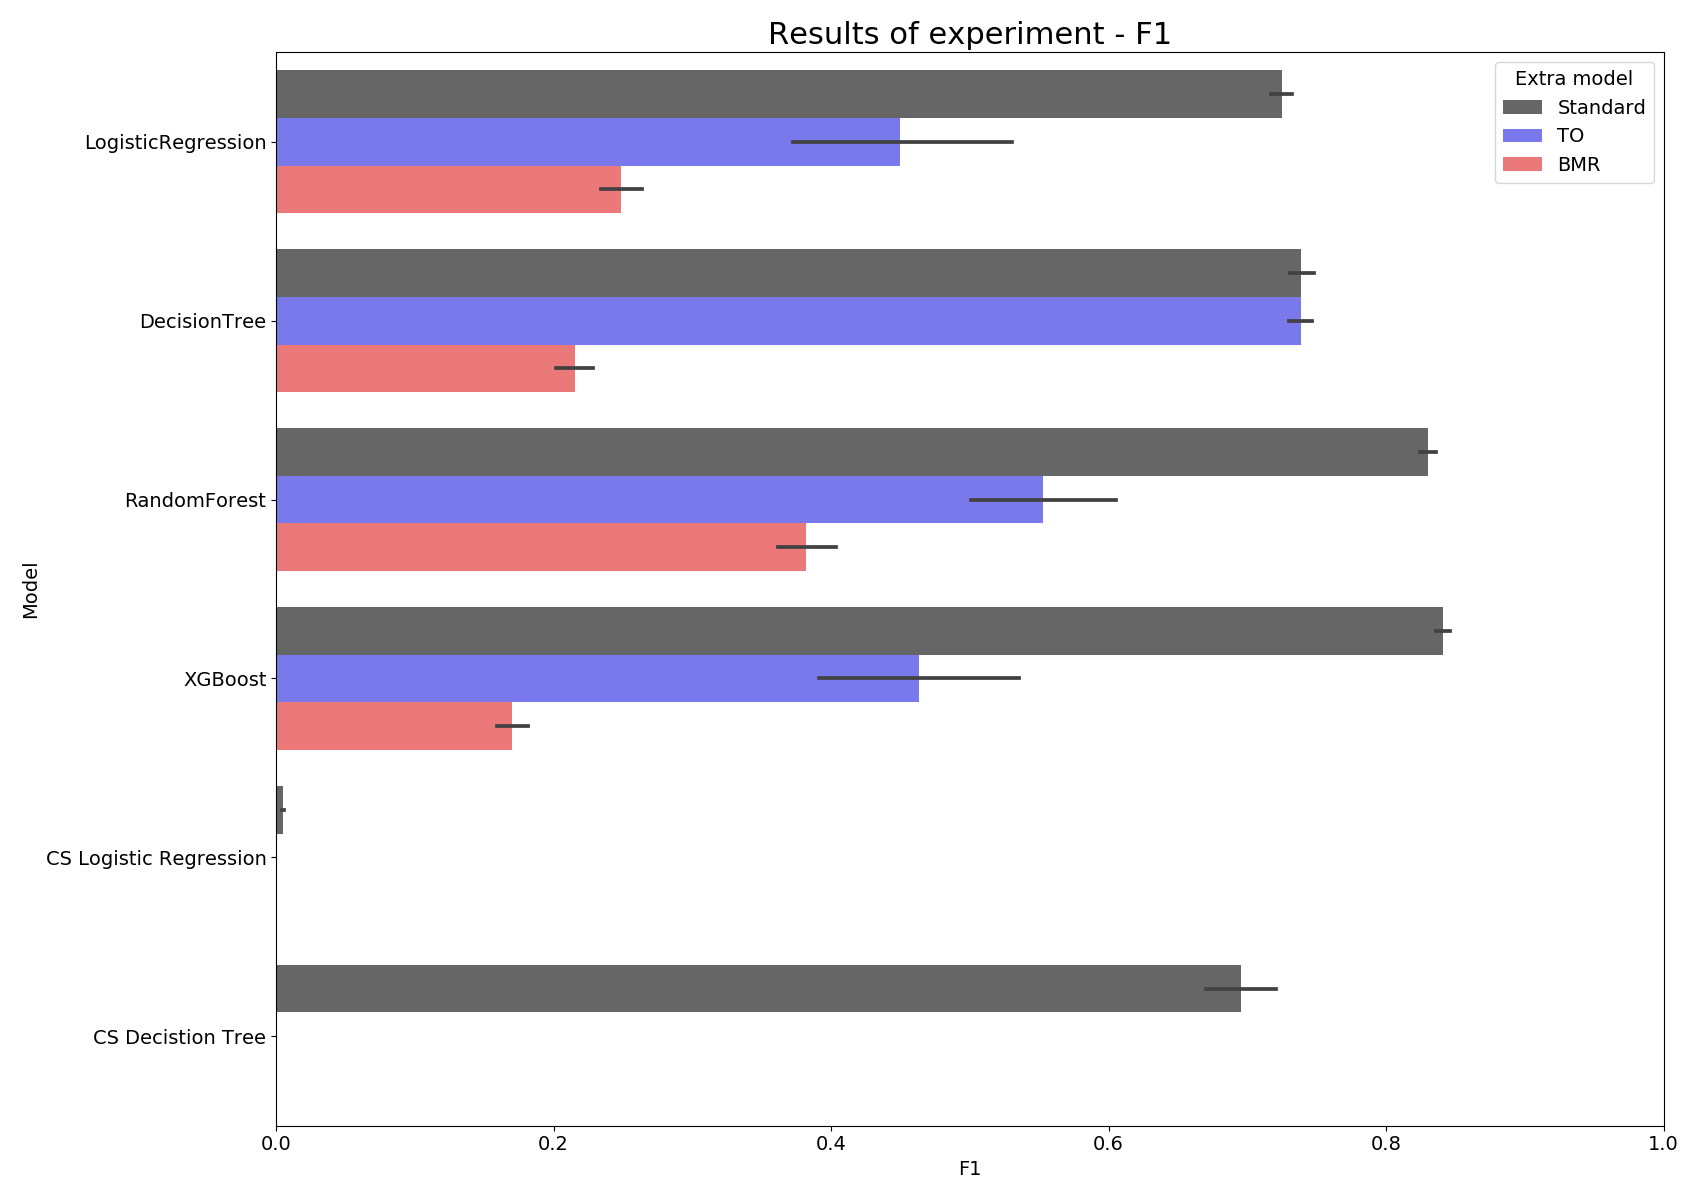
\includegraphics[width=\linewidth]{images/100_config1-F1.png}
	\caption{Wyniki eksperymentu dla miary skuteczności F1-Score. Szare, niebieskie oraz czerwone słupki oznaczają dla pierwszych czterech modeli: regresji logistycznej (LogisticRegression), drzewa decyzyjnego (DecisionTree), lasu losowego (RandomForest) oraz XGBoosta, odpowiednio model standardowy, model optymalizacji progu oraz model wykorzystujący minimalizację ryzyka bayesowskiego. Dla modelu drzewa decyzyjnego wrażliwego na koszt (CS Decision Tree) mamy jedynie jedną wartość. Wysokość słupka reprezentuje wartość średnią z 50 powtórzeń, a długość dołączonej kreski oznacza $\pm$ wartość odchylenia standardowego w odpowiednią stronę. Źródło: Opracowanie własne.}
	\label{fig:results-f1}
\end{figure}

Zestawiając uzyskane rezultaty z obu miar, możemy dojść do wniosku, że jeżeli najważniejszym i jedynym kryterium, które chcemy rozważać w ocenie jakości modelu, są oszczędności, to w przypadku tego zbioru danych najlepszym wyborem jest algorytm XGBoost z minimalizacją ryzyka bayesowskiego. Natomiast, jeżeli poza oszczędnościami, chcemy wziąć także pod uwagę ogólną jakość predykcyjną modelu, to wyniki nie jest aż tak jednoznaczny. W~zależności od przypadku będziemy musieli wybierać pomiędzy ogólną skuteczność a oszczędnościami. Ciekawym wyborem w~tym przypadku może być drzewo decyzyjne wrażliwe na koszt, las losowy lub XGBoost w wersji standardowej. Dodatkową informacją, która mogłaby nam pomóc podjąć decyzję, może być ilość pozytywnych klasyfikacji z~każdego modelu oraz ilość analityków zajmujących się sprawdzaniem oszustw, ponieważ może się okazać, że w wyniku zbyt małej ilości osób nie będziemy w~stanie sprawdzić wszystkich wytypowanych spraw. W~takiej sytuacji model, który typuje mniej transakcji do sprawdzania przy zachowaniu podobnej skuteczności dla obu miar, może okazać się najlepszym wyborem. Z~drugiej strony, jeżeli taka informacja byłaby dostępna na początku modelowania, to wymusiłaby ona dodatkowe założenia oraz inne podejście do procesu doboru miary.

Ponadto pierwsze eksperymenty zostały wykonane również z~wykorzystaniem regresji logistycznej wrażliwej na koszt, natomiast z~nieznanych nam przyczyn (być może błędy implementacyjne) uzyskiwała ona ujemny wynik oszczędności oraz $F_1$~Score bliski zeru. Zatem uzyskane wyniki nie zostały opublikowane w~podsumowaniu eksperymentu, ponieważ nie wnosiły one żadnej użytecznej informacji w kontekście przeprowadzanego wnioskowania. Ponadto poza tokiem przeprowadzonych prac został zrealizowany dodatkowy eksperyment na innym zbiorze danych i~model ten uzyskiwał prawidłowe rezultaty, zatem wina może leżeć także po stronie naszego zbioru danych lub definicji macierzy kosztu.

\chapter*{Podsumowanie}
\addcontentsline{toc}{chapter}{Podsumowanie} \markboth{Podsumowanie}{}
Całość pracy rozpoczęło wprowadzenie problemu detekcji oszustw na kartach kredytowych oraz omówienie aktualnego podejścia do tworzenia systemów wykrywających oszustwa. Następnie omówiono rodzaje miar, które są standardowo wykorzystywane w~statystyce oraz uczeniu maszynowym, a~także miary, które stosuje się w~problemach wrażliwych na koszt. Dalej opisano podstawy teoretyczne standardowych modeli predykcyjnych, ich modyfikacji wrażliwych na koszt oraz klasyfikatorów wrażliwych na koszt. W~ostatniej części pracy przeprowadzono eksperyment, którego celem było porównanie wybranych klasyfikatorów na danych rzeczywistych dotyczących detekcji oszustw na kartach kredytowych.

Na podstawie przeprowadzonego doświadczenia ustalono, że na tym konkretnym zbiorze danych, dzięki wykorzystaniu metod wrażliwych na koszt, można zwiększyć oszczędności w problemie detekcji oszustw na kartach kredytowych. Najlepszym modelem pod tym względem okazał się XGBoost, który do tej pory nie był rozważanych w pracach A.~Bahnsena, które dotyczyły podobnych zagadnień. Dodatkowo zauważono, że wykorzystanie klasyfikatorów wrażliwych na koszt znacząco obniża skuteczność modeli w~sensie standardowych miar. W~przypadku, potrzeby zachowania balansu pomiędzy tymi dwoma miarami, najlepszych wyborem byłby algorytm XGBoost, las losowy lub drzewo decyzyjne wrażliwe na koszt.

Na podstawie przeprowadzonych badań wydaje się, że bardzo ciekawym kierunkiem do dalszych rozważań mogą być metody typu \textit{ensemble}, których klasyfikatorem bazowym byłoby drzewo decyzyjne wrażliwe na koszt. Takie działania zostały już podjęte dla lasów losowych w cytowanej wcześniej pracy A.~Bahnsena~\cite{alej2015ensemble}. Z~uwagi na fakt, że algorytm XGBoost otrzymywał najlepsze rezultaty dla obu miar skuteczności oraz drzewo decyzyjne w wersji wrażliwej na koszt uzyskiwało lepsze rezultaty niż standardowa wersja modelu, daje to nadzieje, że XGBoost wrażliwy na koszt mógłby dawać jeszcze lepsze wyniki.

\appendix

\chapter{Dokładność}
\label{dokladnosc-dd}
W tej części udowodnimy następujący wzór
\begin{equation}
	\label{eq:dokladnosc}
	\text{Dokładność} = \frac{TP + TN}{TP + FP + FN + TN} = \alpha \cdot \text{Czułość} + (1-\alpha) \cdot \text{Swoistość} \text{.}
\end{equation}

Przypomnijmy, że
$$ \alpha = \frac{TP + FN}{TP + FP + FN + TN} \text{,} $$
$$ 1 - \alpha = \frac{TN + FP}{TP + FP + FN + TN} \text{,} $$
$$ \text{Czułość} = \frac{TP}{TP + FN} \text{,} $$
$$ \text{Swoistość} = \frac{TN}{TN + FP} \text{.} $$

Wstawiając do prawej strony równania \ref{eq:dokladnosc} odpowiednie wartości otrzymujemy
$$\frac{TP + FN}{TP + FP + FN + TN} \cdot \frac{TP}{TP + FN} + \frac{TN + FP}{TP + FP + FN + TN} \cdot \frac{TN}{TN + FP} \text{.}$$
Skracając  ułamki otrzymujemy
$$ \frac{TP}{TP + FP + FN + TN} + \frac{TN}{TP + FP + FN + TN} = \text{Dokładność} \text{.} \qed $$


\chapter{Minimalizacja ryzyka bayesowskiego}
\label{bmr-proof}
W niniejszej części dodatku wyprowadzimy wzór 
$$ c_i = 1 \Leftrightarrow P(c_i = 1|\iks_{i}) \ge \frac{C^{(i)}_{1,0} - C^{(i)}_{0,0}}{C^{(i)}_{0,1} - C^{(i)}_{1,1} - C^{(i)}_{0,0} + C^{(i)}_{1,0}} \text{.}$$

Przypomnijmy, że klasyfikujemy daną obserwację jako pozytywną, jeżeli prawdziwa jest  nierówność
\begin{equation}
	\label{decyzja-bmr}
	c_i = 1 \Leftrightarrow R(c_i = 1|\iks_{i}) \leq R(c_i = 0|\iks_{i}) \text{.}
\end{equation}
Ponadto w sekcji \ref{bmr} definiowaliśmy ryzyko klasyfikacji w następujący sposób:
$$ R(c_i = 1|\iks_{i}) = C^{(i)}_{1,1}P(y_i = 1|\iks_{i}) + C^{(i)}_{1,0}P(y_i = 0|\iks_{i}) \text{,}$$
$$ R(c_i = 0|\iks_{i}) = C^{(i)}_{0,1}P(y_i = 1|\iks_{i}) + C^{(i)}_{0,0}P(y_i = 0|\iks_{i}) \text{.}$$
W celu skrócenia zapisu wprowadźmy następujące oznaczenie
$$ P_k = P(y_i = k|\iks_{i}), \quad k \in \{0,1\} \text{.}$$
Korzystając z powyższych oznaczeń, definicji $R(c_i = 1|\iks_{i}), R(c_i = 0|\iks_{i})$ oraz równania \eqref{decyzja-bmr} otrzymujemy
$$ C^{(i)}_{1,1}P_1 +  C^{(i)}_{1,0}P_0 \leq  C^{(i)}_{0,0}P_0 +  C^{(i)}_{0,1}P_1 \text{.}$$
Korzystając z własności 
$$ P_0 = 1 - P_1 \text{,}$$
mamy
$$  C^{(i)}_{1,1}P_1 +  C^{(i)}_{1,0}(1-P_1) \leq  C^{(i)}_{0,0}(1-P_1) +  C^{(i)}_{0,1}P_1 \text{.}$$
Następnie dokonując przekształceń algebraicznych, otrzymujemy
$$  C^{(i)}_{1,0}- C^{(i)}_{0,0} \leq P_1 \cdot ( C^{(i)}_{0,1} -  C^{(i)}_{0,0} -  C^{(i)}_{1,1} +  C^{(i)}_{1,0}) \text{.} $$
Zakładając, że $ C^{(i)}_{0,1} -  C^{(i)}_{0,0} -  C^{(i)}_{1,1} +  C^{(i)}_{1,0} > 0$ ostatecznie otrzymujemy
$$ P_1 \geq \frac{ C^{(i)}_{1,0}- C^{(i)}_{0,0}}{ C^{(i)}_{0,1} -  C^{(i)}_{0,0} -  C^{(i)}_{1,1} +  C^{(i)}_{1,0}}. \qed $$

\chapter{Skrypty}
\label{scripts}
W niniejszej części zostaną zaprezentowane skrypty, które były wykorzystane do przeprowadzenia eksperymentu. Główna część eksperymentu była wykonywana w skrypcie \textit{trainmodels.py}. Był on odpowiedzialny za wczytanie danych oraz konfiguracji, podział danych na odpowiednie podzbiory, a także rozdzielenie obliczeń na kilka wątków procesora. Wyniki z~poszczególnych iteracji eksperymentu były zapisywane do plików \textit{csv}, a~następnie analizowane z~wykorzystaniem notatnika \textit{Jupyter Notebook}.
\lstinputlisting[language=Python, caption={Skrypt \textit{trainmodels.py} odpowiedzialny za główną część eksperymentu.}]{../../train_models.py}

Zdecydowana większość kodu została zawarta w~skrypcie \textit{utils.py} i~została oddzielona od poprzedniego programu, aby ułatwić zarządzanie częścią programistyczną projektu. Składa się on z~funkcji służących między innymi do:
\begin{itemize}
	\item wywoływania skryptu z~poziomu linii komend,
	\item wczytywania plików \textit{json} z~konifugracją,
	\item generowania macierzy kosztu w~odpowiednim formacie,
	\item trenowania modeli,
	\item tworzenia podsumowania wyników.
\end{itemize}
\lstinputlisting[language=Python, caption={Skrypt \textit{utils.py} zawierający funkcje pomocnicze do głównej części eksperymentu.}]{../../src/utils.py}

Eksperyment uruchamiano za pomocą skryptu \textit{trainmodels.sh}, który wykonywał skrypt \textit{trainmodels.py} z~odpowiednimi argumentami.
\lstinputlisting[language=bash, caption={Skrypt \textit{trainmodels.sh} odpowiedzialny za uruchamianie eksperymentu.}]{../../train_models.sh}

\backmatter
\nocite{*}

\bibliografia{references} 
\markboth{Bibliografia}{}

\end{document}